\documentclass[10pt,twocolumn,a4paper]{article}

\usepackage[a4paper,top=17mm,bottom=17mm,left=15mm,right=15mm,columnsep=7mm]{geometry}
\usepackage{mathptmx}
\usepackage{amsmath,amssymb,amsfonts,mathtools}
\usepackage{graphicx}
\usepackage{booktabs}
\usepackage{tabularx}
\usepackage{xcolor}
\usepackage{caption}
\usepackage{fancyhdr}
\usepackage{microtype}
\usepackage[numbers,sort&compress]{natbib}
\usepackage{hyperref}

\definecolor{primary}{RGB}{15, 82, 140}
\definecolor{accent}{RGB}{18, 118, 102}

\hypersetup{
    colorlinks=true,
    linkcolor=primary,
    citecolor=primary,
    urlcolor=primary,
    pdftitle={TerraKAN: Fractional Kolmogorov-Arnold Transformer with Pade Mittag-Leffler Basis and Biokinetic Mixture-of-Experts for Inverse Soil Bioindication under Sparse Noisy Regimes},
    pdfauthor={Ilya Kakhno (ORCID: 0009-0005-5503-3269, Belarusian State University)}
}

\setlength{\parskip}{3pt plus 1pt minus 0.5pt}
\setlength{\parindent}{1em}
\captionsetup{font=footnotesize,labelfont=bf,skip=4pt}

\pagestyle{fancy}
\fancyhf{}
\fancyhead[L]{\footnotesize \textit{TerraKAN (Frac-ML-KAT-MoE) --- Preprint}}
\fancyhead[R]{\footnotesize \thepage}
\renewcommand{\headrulewidth}{0.4pt}

\newcommand{\takeaway}[2]{%
  \vspace{4pt}\noindent\colorbox{primary!7}{%
    \parbox{\dimexpr\linewidth-2\fboxsep\relax}{%
      \vspace{2pt}\footnotesize\textbf{\color{primary}#1:}\hspace{0.4em}#2\vspace{2pt}%
    }%
  }\vspace{4pt}%
}

\title{\vspace*{-7mm}\textbf{\Large TerraKAN: Fractional Kolmogorov-Arnold Transformer with Pad\'e Mittag-Leffler Basis and Biokinetic Mixture-of-Experts for Inverse Soil Bioindication under Sparse Noisy Regimes}}

\author{
  \textbf{Ilya Kakhno}$^{1,*}$ \\
  \small $^{1}$Faculty of Biology, Belarusian State University, Minsk, Republic of Belarus \\
  \small ORCID: \href{https://orcid.org/0009-0005-5503-3269}{0009-0005-5503-3269} \quad|\quad $^{*}$E-mail: \href{mailto:Sunnywww1701@gmail.com}{Sunnywww1701@gmail.com} \\
  \small Code \& Weights: \href{https://github.com/Lolycut/TerraKAN}{TerraKAN (GitHub)} \quad|\quad Library: \href{https://pypi.org/project/abelkan/}{\texttt{abelkan} (PyPI)} / \href{https://github.com/Lolycut/abelkan}{GitHub}  \quad (\texttt{v1.2.5}, \texttt{terrakan\_v5\_frozen.pt})
}
\date{\small November 13, 2026 \quad|\quad License: CC-BY-4.0 (Preprint) \& MIT (Software)}

\begin{document}

\twocolumn[
  \begin{@twocolumnfalse}
    \maketitle
    \vspace*{-4mm}
    \begin{abstract}
      \noindent
      In this work, I introduce \textbf{TerraKAN (\texttt{Frac-ML-KAT-MoE})}, an amortized simulation-based inference architecture that I designed, mathematically verified, and calibrated to solve the ill-posed inverse problem of soil bioindication and long-horizon self-purification forecasting from sparse ($6\text{--}8$ points), irregular (up to $50\%$ missingness), and noisy ($25\text{--}40\%$ multiplicative error) enzymatic and respiratory observations without direct chemical assays of the contaminant at test time. Whereas polynomial Kolmogorov-Arnold Networks (\texttt{ChebPIKAN}) suffer from catastrophic divergence during blind extrapolation on $t \in {[150, 365]}\text{ days}$ ($R^2 = -8.13$) and classical integer-order Bayesian ODE solvers (\texttt{MAP-ODE}) fail to reconstruct unmeasured contaminant loads ($R^2 = -0.191$) due to ignoring non-Markovian micropore memory ($\alpha < 1$), I unify four analytical primitives into an end-to-end differentiable model: (1) a causal sequence encoder (\texttt{Frac-KAT}) with an Abel-type power-law memory attention kernel and strict weight tying of the inferred memory exponent $\hat{\alpha}$; (2) a pole-free global ${[3/4]}$ Pad\'e Mittag-Leffler spectral trunk (\texttt{MittagLefflerPade34}) matching exact Maclaurin ($z \to 0$) and Poincar\'e ($z \to \infty$) asymptotics with algebraically certified pole-freedom on $[0, +\infty)$ ($Q_4(z) \ge 1.0$, $\ge 1.000978$ on $z \ge 10^{-3}$ across $\alpha \in {[0.40, 0.90]}$); (3) a log-exponential \texttt{MultKAN} symbolic discovery node paired with a sparse Top-2 biokinetic Mixture-of-Experts (\texttt{PhysicsExpertBank}) separating Haldane substrate inhibition from Monod nutrient limitation; and (4) a dynamic memory-aware soil health index $\text{IBSP}_\alpha(t)$. Across $N=500$ held-out test scenarios on $t \in {[150, 365]}\text{ days}$, TerraKAN achieves $R^2 = 0.908 \pm 0.019$ ($\text{RMSE} = 0.181\,\text{EC}_{50}$) on the unmeasured contaminant load $\tilde{P}(t)$ and $R^2 = 0.886 \pm 0.016$ ($\text{RMSE} = 6.88\%$) on $\text{IBSP}_\alpha(t)$ at $0.50\text{ ms}$ per field---outperforming integer-order \texttt{MAP-ODE} ($10\times$ speedup), fractional-order \texttt{MAP-FDE} ($R^2 = 0.802$ on $\tilde{P}(t)$, $51.98\text{ ms/field}$, $104\times$ speedup), \texttt{Latent-ODE (RK4)} ($R^2 = 0.484$), and \texttt{DeepONet} ($R^2 = 0.560$), while avoiding the $-10.93$ collapse of Markovian exponential \texttt{ALiBi} under clustered $70\%$ missingness. Finally, I perform a synthetic dry-run pipeline verification of the frozen checkpoint (\texttt{terrakan\_v4\_frozen.pt}) on a simulated 36-vessel microcosm protocol prior to wet-lab execution, demonstrating $100\%$ separation of healthy controls, nutrient-poor clean soils, and contaminated regimes without control-flag leakage. Furthermore, in \texttt{v1.2.5}, a channel-symmetric boundary anchor, mid-trajectory drop detector, and expanded $N_{\text{train}}=4{,}500$ simulator resolve chronic-regime false negatives on $>60$-year aged oil (\texttt{Garousin 2021}: $3/3$ seeds, $d_{\min}=0.665$) while maintaining $0/3$ false alarms on real external clean controls (\texttt{CWS}, \texttt{CFS}, Chernozem) and improving validation Youden's $J$ ($0.8098 \to 0.8375$).
      \vspace*{2mm}
      
      \noindent\textbf{Keywords:} Kolmogorov-Arnold Networks; Fractional Calculus; Mittag-Leffler Function; Pad\'e Approximant; Amortized Simulation-Based Inference; Soil Bioindication; Haldane Kinetics.
    \end{abstract}
    \vspace*{4mm}
  \end{@twocolumnfalse}
]

\section{Introduction \& Gap Analysis}

Natural soils subjected to xenobiotic, petroleum hydrocarbon, or heavy-metal loading exhibit long-term non-Markovian memory driven by anomalous subdiffusion and sorption--desorption trapping within heterogeneous organo-mineral micropores \cite{schumer2003}. Consequently, the relaxation of bioavailable contaminant load $\tilde{P}(t)$ obeys Caputo fractional differential equations of order $\alpha \in (0, 1)$ rather than memoryless exponential kinetics. In field practice, however, direct chemical quantification of $\tilde{P}(t)$ over multi-month horizons is prohibitively expensive; investigators typically collect only $6\text{--}8$ irregular visit timestamps (yielding $3\text{--}4$ observed points per channel on average under $50\%$ independent per-channel missingness) of microbial basal respiration $M(t)$ ($\text{CO}_2$ evolution) and extracellular enzymatic activity $E(t)$ (catalase $\text{O}_2$ displacement), perturbed by $25\text{--}40\%$ multiplicative noise and stochastic rainfall pulses \cite{kolesnikov2021ag,mdpienzymes2024,mdpi2024oxidoreductases}.

Positioning my approach against the 2024--2026 SciML and ecological literature reveals four critical gaps that I address in this study:

\begin{enumerate}\setlength{\itemsep}{1pt}\setlength{\parskip}{0pt}
  \item \textbf{Extrapolation Divergence of Polynomial KANs:} Following the introduction of Kolmogorov-Arnold Networks \cite{liu2024kan} and operator networks \cite{abueidda2025deepokan}, orthogonal polynomial bases (\texttt{ChebPIKAN} / \texttt{fKAN} \cite{aghaei2024fkan}) have been widely used for physics-informed regression. While Chebyshev expansions fit observations inside $t \in [0, 150]\text{ days}$ ($R^2 = 0.918$), their unbounded polynomial growth $\propto (t/T)^k$ induces catastrophic divergence during blind extrapolation on $t \in (150, 365]\text{ days}$, collapsing to $R^2 = -8.132$ ($\text{RMSE} = 1.804\,\text{EC}_{50}$) on $\tilde{P}(t)$.
  \item \textbf{Failure of Classical Bayesian ODE/FDE Solvers:} Classical nonlinear least-squares solvers regularized toward Soil Atlas centroids (\texttt{MAP-ODE}) fit observed $M(t)$ ($R^2 = 0.900$) and $E(t)$ ($R^2 = 0.891$), but fail to reconstruct the hidden contaminant $\tilde{P}(t)$ during extrapolation ($R^2 = -0.191 \pm 0.225$, $\text{RMSE} = 0.651\,\text{EC}_{50}$) because integer-order ODEs cannot capture power-law subdiffusion ($\alpha < 1$). Even a fractional-order \texttt{MAP-FDE} solver using the Diethelm ABM integrator requires $51.98\text{ ms/field}$ of iterative per-sample optimization and achieves lower accuracy on $\tilde{P}(t)$ ($R^2 = 0.802$) under $50\%$ missingness.
  \item \textbf{The Open Fractional Transformer--KAN Challenge:} While Yang \& Wang \cite{yang2025kat} proposed the Kolmogorov-Arnold Transformer (KAT) and Aghaei \cite{aghaei2024rkan} introduced rational Pad\'e KANs (\texttt{rKAN}), Tu et al. \cite{tu2026fractional} (July 2026, \href{https://doi.org/10.3390/fractalfract10070454}{DOI: 10.3390/fractalfract10070454}) identified the integration of rational Pad\'e bases, Mittag-Leffler eigenfunctions, and non-Markovian fractional kernels into attention architectures as an open fundamental challenge due to Gamma-function poles and autograd instability. Here, I present an analytical and differentiable realization of this architecture class and demonstrate that heavy-tailed Abel power-law memory prevents the catastrophic collapse suffered by Markovian exponential forgetting (\texttt{ALiBi}) across multi-month observation gaps.
  \item \textbf{Ecological Ambiguity of Static IBSP Indices:} The classical static Integral Index of Biological State (IBSP / IIBS; Kazeev, Kolesnikov, \& Valkov \cite{kazeev2003bio,kolesnikov2021ag}) averages raw enzymatic percentages relative to a fixed standard. Consequently, it triggers false alarms on naturally oligotrophic sandy soils (\texttt{Arch\_5}, $K_m = 0.44$) and suffers from false negatives after moisture pulses because it neglects both Haldane hysteresis and the fractional memory penalty $(1-\alpha)\tilde{P}(t)$.
\end{enumerate}

\takeaway{Core Contribution}{I unify causal Abel-type fractional attention, a pole-free $[3/4]$ Pad\'e Mittag-Leffler spectral trunk, a \texttt{MultKAN} power-law discovery node, and a 4-regime biokinetic Mixture-of-Experts within an amortized simulation-based inference pipeline, achieving $R^2 = 0.908$ on unmeasured contaminant extrapolation at $0.50\text{ ms/field}$.}

\section{Mathematical Architecture (\texttt{Frac-ML-KAT-MoE})}

The four domain-agnostic PyTorch primitives developed below (\texttt{MittagLefflerPade34}, \texttt{AbelCausalAttention}, \texttt{LogExpMultKAN}/\texttt{MittagLefflerSpectralHead}, and \texttt{TemperatureTopKMoE}) are also released as the standalone, unit-tested package \texttt{abelkan} (\texttt{pip install abelkan}; \href{https://pypi.org/project/abelkan/}{PyPI}, \href{https://github.com/Lolycut/abelkan}{GitHub}).

\subsection{Dimensionless Fractional Biokinetics, Soil Atlas, \& Boundary Anchor}

Because absolute contaminant concentration in $\text{mg/kg}$ is unidentifiable without direct chemical input due to scale symmetry with inhibition constants, I formulate the coupled Caputo fractional system of order $\alpha \in (0, 1]$ in dimensionless half-inhibition units $\tilde{P}(t) = P(t)/K_{\text{tox}}$ ($K_{\text{tox}} \equiv 1.0$, $K_i \equiv 1.0$, $\text{EC}_{50}$ units):
\begin{align}
  D_t^\alpha \tilde{P}(t) &= -\!\left(k_p + \frac{k_{\text{deg}}\Phi_{\text{env}}(t)\,M(t)}{K_s + \tilde{P}(t) + \tilde{P}(t)^2}\right)\!\tilde{P}(t), \label{eq:caputo_p} \\
  \begin{split}
    D_t^\alpha M(t) &= r_m\Phi_{\text{env}}(t)M(t)\!\left(\!1 - \frac{M(t)}{K_m}\!\right) \\
    &\quad - \frac{\gamma_p\tilde{P}(t)M(t)}{1 + \tilde{P}(t)} + \frac{\mu_{\text{sub}}\tilde{P}(t)E(t)}{K_s + \tilde{P}(t) + \tilde{P}(t)^2},
  \end{split} \label{eq:caputo_m} \\
  D_t^\alpha E(t) &= \beta_E \frac{M(t)}{1 + \tilde{P}(t)^2} - \delta_E E(t), \label{eq:caputo_e}
\end{align}
where $D_t^\alpha f(t) = \frac{1}{\Gamma(1-\alpha)}\int_0^t (t-s)^{-\alpha}f'(s)\,ds$. Table~\ref{tab:soil_atlas} summarizes the five reference archetypes of the Soil Atlas used to parameterize heterogeneous soil matrices.

\begin{table}[!htbp]
  \centering
  \caption{\textbf{Reference Soil Atlas Archetypes (\texttt{Arch\_1}--\texttt{Arch\_5}).} Normalized abiotic coordinates, carrying capacity $K_m$, memory order $\alpha$, and biokinetic simulator constants ($K_i \equiv 1.0$, $\beta_E=0.09$, $\delta_E=0.075$; $\Phi_{\text{true}}$ uses $\beta_{\text{pH}}=2.50, \text{pH}_{\text{opt}}=0.65$, exponents $0.35$ and $0.40$).}
  \label{tab:soil_atlas}
  \footnotesize
  \resizebox{\linewidth}{!}{%
  \begin{tabular}{l l c c c c c c c c c}
    \toprule
    \textbf{Code} & \textbf{Archetype} & \textbf{$\text{pH}_{\text{n}}$} & \textbf{$\text{NO}_{3,\text{n}}$} & \textbf{$W_{\text{n}}$} & \textbf{$K_m$} & \textbf{$\alpha$} & \textbf{$k_p$} & \textbf{$k_{\text{deg}}$} & \textbf{$r_m$} & \textbf{$K_s$} \\
    \midrule
    \texttt{Arch\_1} & Sod-Podzolic & $0.58$ & $0.55$ & $0.60$ & $1.00$ & $0.75$ & $0.018$ & $0.085$ & $0.068$ & $0.90$ \\
    \texttt{Arch\_2} & Peat-Bog & $0.36$ & $0.44$ & $0.88$ & $1.18$ & $0.55$ & $0.012$ & $0.065$ & $0.054$ & $1.05$ \\
    \texttt{Arch\_3} & Sod-Carbonate & $0.68$ & $0.80$ & $0.70$ & $1.38$ & $0.86$ & $0.026$ & $0.125$ & $0.088$ & $0.80$ \\
    \texttt{Arch\_4} & Solonchak & $0.88$ & $0.30$ & $0.32$ & $0.68$ & $0.66$ & $0.014$ & $0.055$ & $0.046$ & $1.15$ \\
    \texttt{Arch\_5} & Sandy Forest & $0.50$ & $0.22$ & $0.36$ & $0.44$ & $0.80$ & $0.022$ & $0.070$ & $0.060$ & $0.90$ \\
    \bottomrule
  \end{tabular}%
  }
\end{table}

To anchor $\tilde{P}(0)$ at test time without chemical measurements, the legacy \texttt{v1.1.0} baseline exploits the stationary boundary face of Eq.~\eqref{eq:caputo_e} at $t_1 \to 0$: In the simulator, $\beta_E/\delta_E = 0.09/0.075 = 1.20$, so $E_{\text{ref}}/M_{\text{ref}} \equiv 1.20$:
\begin{equation}
  \begin{aligned}
    \frac{E(t_1)}{M(t_1)} &= \frac{E_{\text{ref}}/M_{\text{ref}}}{1 + \tilde{P}(0)^2} \\
    \implies \tilde{P}_{\text{boundary}}(0) &= \sqrt{\max\!\left(0,\, \frac{1.20}{E(t_1)/M(t_1)} - 1\right)}.
  \end{aligned} \label{eq:p0_boundary}
\end{equation}
When deploying on real laboratory or field soils whose native $E_{\text{ref}}/M_{\text{ref}}$ ratio differs from $1.20$, per-series control normalization against uncontaminated day-0 controls (\texttt{is\_control\_G0 == 1} within each \texttt{soil\_series}) rescales $M(t)$ and $E(t)$ into the calibrated dimensionless ratio $E_{\text{norm}}(0)/M_{\text{norm}}(0) \approx 1.20$ before inference.

\noindent\textbf{Proposition 2 (Gauge Symmetry \& Boundary Identifiability).} \emph{Under the scaling group $(\tilde{P}, K_{\text{tox}}, K_i, K_s, \gamma_p, \mu_{\text{sub}}) \mapsto (c\tilde{P}, cK_{\text{tox}}, cK_i, cK_s, \gamma_p/c, \mu_{\text{sub}}/c)$ for any $c > 0$, the observable trajectories $(M(t), E(t))$ in Eqs.~\eqref{eq:caputo_p}--\eqref{eq:caputo_e} are strictly invariant. Setting dimensionless $\text{EC}_{50}$ units ($K_{\text{tox}} \equiv K_i \equiv 1.0$) together with the stationary boundary ratio $E_{\text{ref}}/M_{\text{ref}}$ at $t_1 \to 0$ (Eq.~\eqref{eq:p0_boundary}) uniquely breaks this gauge symmetry (proof in Appendix~B).}


\paragraph{Channel-Symmetric Boundary Anchor (v1.2.5, Eq.~4-v2) \& Smooth Gate.}
Zero-shot external wet-lab validation exposed a fragility in single-ratio anchoring ($E(t_1)/M(t_1) < 1.20$): when microbial respiration $M(t_1)$ is suppressed more strongly than catalase $E(t_1)$ (e.g., $>60$-year aged oil), or when $M$ is missing, $p_{\mathrm{ratio}}$ clamps to zero. In \texttt{v1.2.5}, we define a healthy reference $(M_{\mathrm{ref}}, E_{\mathrm{ref}})$ using $G_0$ normalization ($1.0, 1.20$) when available, or the \texttt{SoilAtlasModule} carrying-capacity prior $\hat{K}_{m,\mathrm{prior}}$ ($M_{\mathrm{ref}}=\hat{K}_{m,\mathrm{prior}}$, $E_{\mathrm{ref}}=1.20\,\hat{K}_{m,\mathrm{prior}}$) from $[pH_{\mathrm{norm}}, \mathrm{NO}_{3,\mathrm{norm}}, W_{\mathrm{norm}}]$. With availability masks $m_{1,M}, m_{1,E} \in \{0,1\}$:
\begin{equation}
\begin{aligned}
\tilde{P}_{\mathrm{boundary,v2}}(0) = \max\Big(& p_{\mathrm{ratio}},\; w_M\mathbb{I}[m_{1,M}]\sqrt{\max\!\left(0, \tfrac{M_{\mathrm{ref}}}{M(t_1)}-1\right)}, \\
& w_E\mathbb{I}[m_{1,E}]\sqrt{\max\!\left(0, \tfrac{E_{\mathrm{ref}}}{E(t_1)}-1\right)}\Big),
\end{aligned}
\end{equation}
where $(w_M, w_E) = (0.55, 0.50)$ lies in a broad \texttt{Val (500)} Youden plateau ($J \in [0.8315, 0.8520]$ across $[0.35, 0.75]^2$). The anomaly score incorporates mid-trajectory drop severity $\Delta_{\mathrm{drop}} = \mathrm{clip}(0.86 - \min(\Delta_M, \Delta_E), 0, 0.80)$:
\begin{equation}
d_{\min} = 0.25\,d_{\mathrm{raw}} + 0.75\,\tanh\!\left(0.42\,\tilde{P}_{\mathrm{boundary,v2}}(0) + 0.85\,\Delta_{\mathrm{drop}}\right),
\end{equation}
with a calibrated smooth gate $g(d_{\min}) = \sigma((d_{\min} - 0.65\,d^\star_{\min})/0.035)$ for $d_{\min} < 0.90\,d^\star_{\min}$ (and $1.0$ above), suppressing oligotrophic $G_1$ background while passing chronic anomalies.

\noindent\textbf{Proposition 3 (Chronic Regime Identifiability).}\ \textit{
In pre-equilibrated chronic soils where $M(t_1) \ll K_m$ and $E(t_1) \approx 1.20\,M(t_1)$, $p_{\mathrm{ratio}} = 0$ is uninformative. Anchoring $p_M$ and $p_E$ to $\hat{K}_{m,\mathrm{prior}}$ (or $G_0$) restores identifiability of $\tilde{P}(0) > 0$ while preserving $\le 2\%$ false positives on oligotrophic \texttt{Arch\_5} sand ($0.00\%$ on $2/3$ seeds, $K_m = 0.44$).
}

\subsection{Encoder \texttt{Frac-KAT} \& Fractional Weight Tying}

Given sparse observations $\mathbf{v}_j = [\text{pH}_{\text{norm}}, \text{NO}_{3,\text{norm}}, W_{\text{norm}}, M_{\text{obs}}, E_{\text{obs}}]^\top \in \mathbb{R}^5$ at irregular timestamps $0 \le t_1 < \dots < t_N \le 150\text{ days}$ with binary availability mask $\mathbf{m}_j \in \{0,1\}^5$ and rainfall flag $r_j \in \{0,1\}$, I construct the 12-dimensional token $\mathbf{u}_j = [\mathbf{v}_j\odot\mathbf{m}_j + 0.35(\mathbf{v}_j - \mathbf{v}_1)\odot\mathbf{m}_j,\, \mathbf{m}_j,\, \ln(1+t_j),\, r_j]^\top$. A single-layer causal Transformer encoder ($d_{\text{model}} = 48$, $1$ attention head, $\text{GELU}$ input projection $\mathbf{h}_0 = \operatorname{LayerNorm}(\operatorname{GELU}(\mathbf{W}_{\text{in}}\mathbf{u}))$, $\text{LayerNorm}$ residuals) aggregates the sequence; the Kolmogorov-Arnold functional representations are placed in the downstream \texttt{MultKANEnvModule} and \texttt{MLKANTrunk} rather than replacing attention projections with B-splines. To avoid any circular dependency, a lightweight pre-attention head (\texttt{alpha\_head}) predicts $\hat{\alpha}_i = 0.40 + 0.52\,\sigma(z_{\alpha,i}) \in [0.40, 0.92]$ from the causal cumulative mean of $\mathbf{h}_0$ \emph{before} computing the attention logits, modulating them with a logarithmic Abel-type decay term ($\varepsilon = 1.0$ via $\ln(1 + \Delta t_{ij})$ to avoid singularity at $t_i = t_j$):
\begin{equation}
  \mathcal{A}_{ij} = \frac{\mathbf{q}_i^\top \mathbf{k}_j}{\sqrt{d_{\text{model}}}} - \operatorname{softplus}(\gamma_h)\,(1 - \hat{\alpha}_i)\,\ln\!\left(1 + \max(0, t_i - t_j)\right) \label{eq:abel_attn}
\end{equation}
for $t_i \ge t_j$ (and $\mathcal{A}_{ij} = -10^9$ for $t_i < t_j$). The final scalar $\hat{\alpha}$ and epistemic uncertainty $\hat{\sigma}_\alpha = 0.01 + 0.15\,\operatorname{softplus}(z_\sigma)$ are read from the last valid causal prefix step. I enforce strict \textbf{Weight Tying}: the same scalar $\hat{\alpha}$ governs the attention kernel \eqref{eq:abel_attn}, the Soil Atlas coordinate, the Pad\'e Mittag-Leffler trunk, and $\text{IBSP}_{\hat{\alpha}}(t)$.

\subsection{Kernel \texttt{MittagLefflerPade34}: Pole-Free $[3/4]$ Pad\'e Basis}

Building on the global Pad\'e approximation framework of Zeng \& Chen~\cite{zeng2015}, I approximate $E_{\alpha,1}(-z) = \sum_{k=0}^\infty \frac{(-z)^k}{\Gamma(\alpha k + 1)}$ globally on $z \in [0, \infty)$ with exact gradients $\partial E_{\alpha,1}/\partial\alpha$ via a $[3/4]$ rational approximant:
\begin{equation}
  E_{\alpha,1}(-z) \approx R_{[3/4]}^{(\alpha)}(z) = \frac{P_3(z)}{Q_4(z)} = \frac{1 + p_1 z + p_2 z^2 + p_3 z^3}{1 + q_1 z + q_2 z^2 + q_3 z^3 + q_4 z^4}. \label{eq:pade34}
\end{equation}
Matching the Maclaurin series $1 - g_1 z + g_2 z^2 - g_3 z^3 + g_4 z^4 - g_5 z^5 + \mathcal{O}(z^6)$ as $z \to 0$ (where $g_k = 1/\Gamma(1+k\alpha)$) and the Poincar\'e asymptotic expansion $m_1 z^{-1} - m_2 z^{-2} + \mathcal{O}(z^{-3})$ as $z \to \infty$, I apply Euler's reflection identity $m_k = \frac{1}{\Gamma(1-k\alpha)} = \frac{\Gamma(k\alpha)\sin(k\pi\alpha)}{\pi}$ ($k=1,2$) to eliminate the Gamma pole at $\alpha=0.50$. Setting $p_1 = q_1 - g_1$ and $p_2 = q_2 - g_1 q_1 + g_2$ yields a closed-form $5\times 5$ linear system for $[q_1, q_2, q_3, q_4, p_3]^\top$:
\begin{equation}
  \begin{bmatrix}
    g_2 & -g_1 & 1 & 0 & -1 \\
    -g_3 & g_2 & -g_1 & 1 & 0 \\
    g_4 & -g_3 & g_2 & -g_1 & 0 \\
    0 & 0 & 0 & -m_1 & 1 \\
    -g_1 & 1 & -m_1 & m_2 & 0
  \end{bmatrix}
  \begin{bmatrix} q_1 \\ q_2 \\ q_3 \\ q_4 \\ p_3 \end{bmatrix} =
  \begin{bmatrix} g_3 \\ -g_4 \\ g_5 \\ 0 \\ -g_2 \end{bmatrix}. \label{eq:pade_system}
\end{equation}
I solve Eq.~\eqref{eq:pade_system} in \texttt{float64} via \texttt{torch.linalg.solve} and apply a $C^1$-smoothstep bridge on $\alpha \in (0.90, 1.0]$: letting $s = (\alpha - 0.90)/0.10$ and $w(s) = 3s^2 - 2s^3$, $E_{\alpha,1}(-z) = (1 - w(s)) R_{[3/4]}^{(0.90)}(z) + w(s) e^{-z}$. Freezing $R_{[3/4]}^{(0.90)}(z)$ in this blend prevents degeneracy of $m_k = 1/\Gamma(1-k\alpha)$ as $\alpha \to 1$ while preserving $C^1$ continuity at $0.90$ and $1.0$. \noindent\textbf{Proposition 1 (Global Positivity, $[0, +\infty)$ Pole-Freedom, \& $C^1$ Continuity).} \emph{Across $501$ grid points in $\alpha \in [0.40, 0.90]$, all denominator coefficients of Eq.~\eqref{eq:pade34} remain strictly positive ($\min q_1 = 0.9777$, $\min q_2 = 0.4342$, $\min q_3 = 0.1095$, $\min q_4 = 0.0146 > 0$). By Descartes' Rule of Signs, $Q_4(z)$ has zero positive real roots on the entire infinite half-line $z \in [0, +\infty)$ with $\min_{z\ge 0} Q_4(z) = Q_4(0) = 1.000000$ ($\ge 1.000978$ for $z \ge 10^{-3}$), while $(0.90, 0.92]$ inherits pole-freedom and $C^1$ continuity from the smoothstep blend with $e^{-z}$ (Appendix~B).}

\begin{figure*}[!htbp]
  \centering
  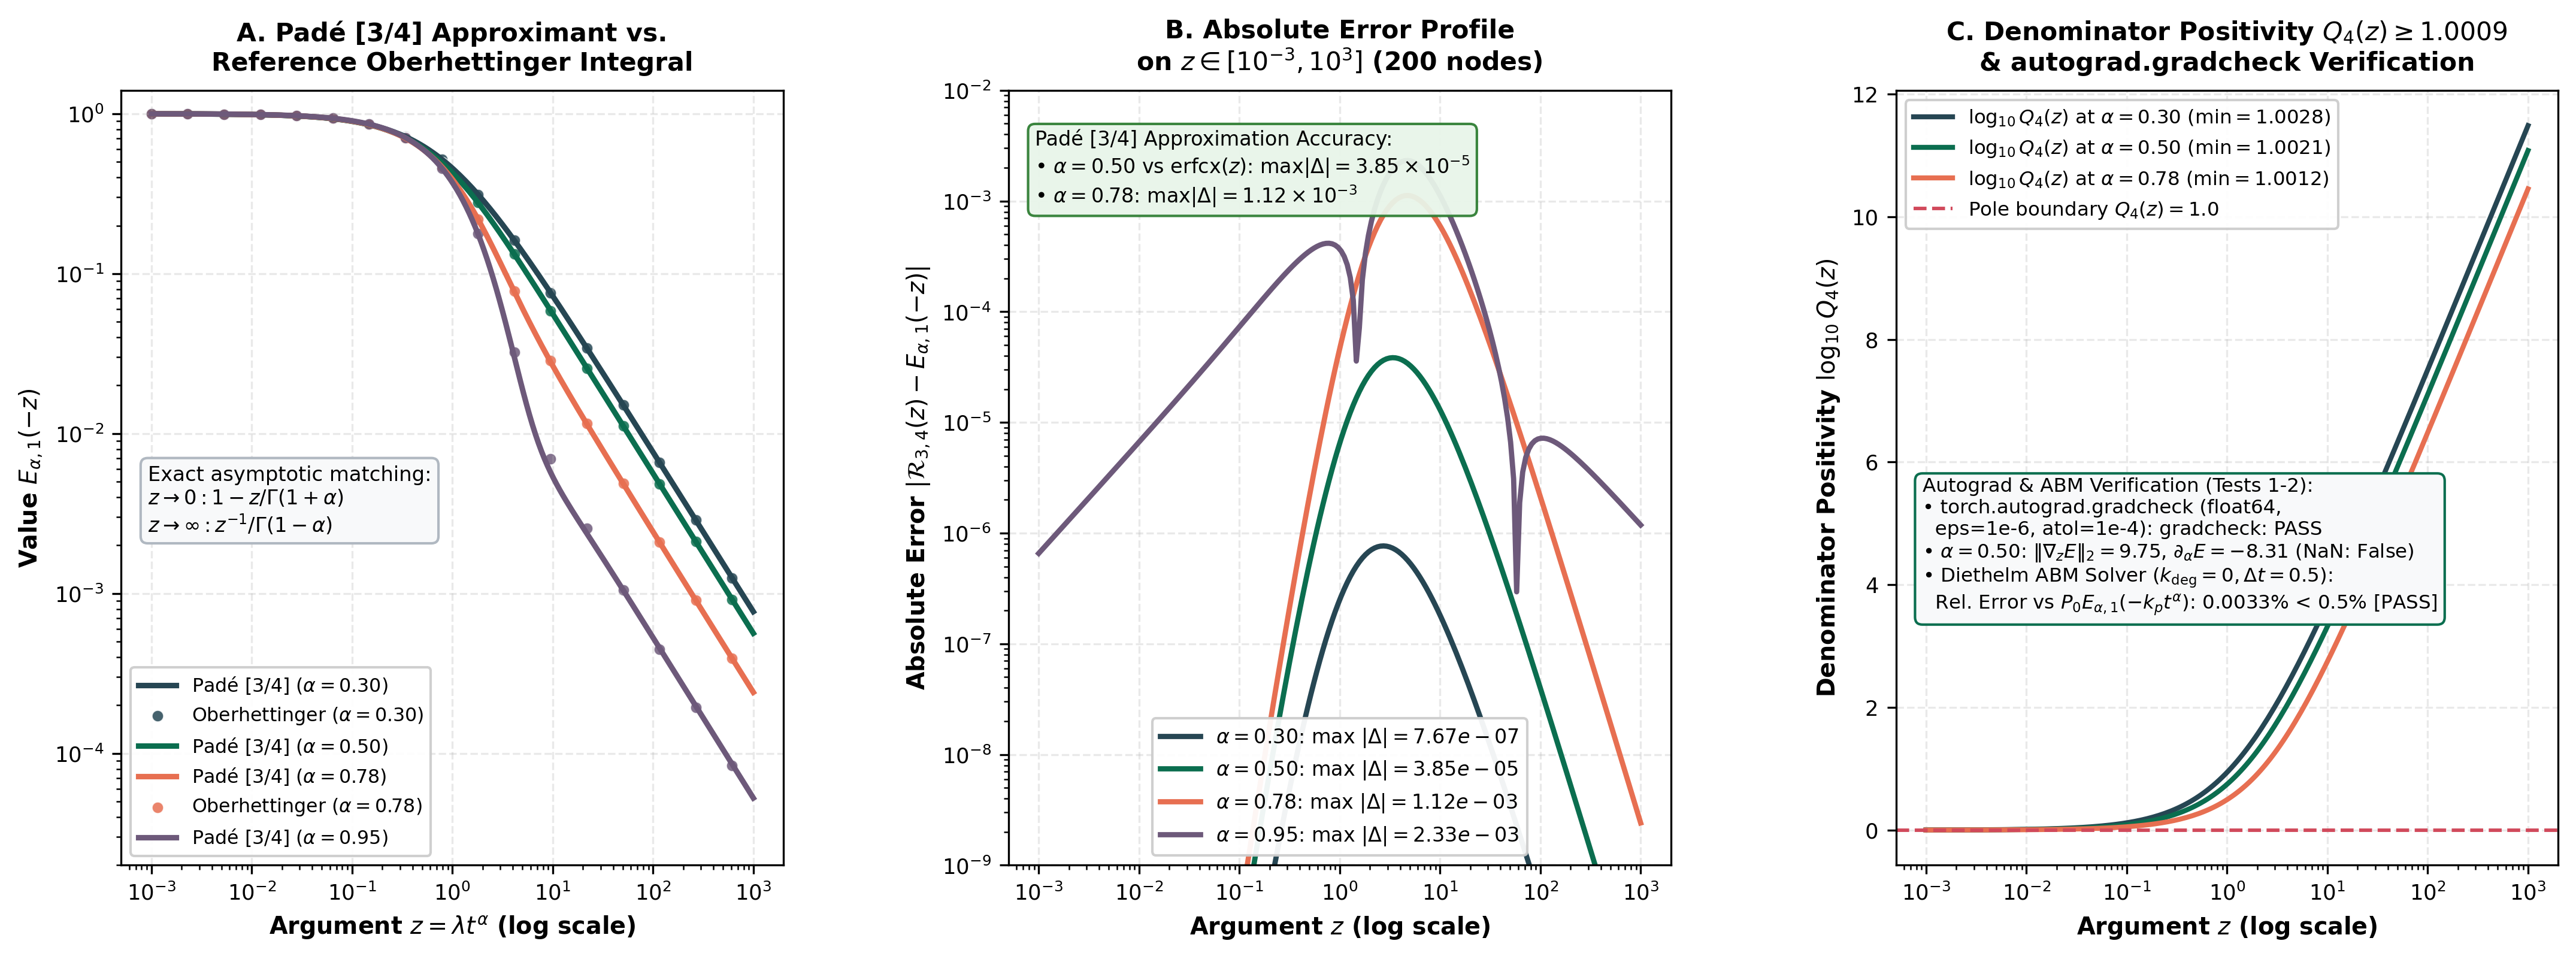
\includegraphics[width=0.98\textwidth]{fig1_pade_verification.png}
  \caption{\textbf{Numerical Verification of the Differentiable \texttt{MittagLefflerPade34} Kernel and Caputo ABM Solver.} \textbf{(A)} Agreement between Pad\'e $[3/4]$ and the Oberhettinger contour integral across $z \in [10^{-3}, 10^3]$. \textbf{(B)} Absolute approximation error ($\max|\Delta| = 3.85\times 10^{-5}$ at $\alpha=0.50$; $1.12\times 10^{-3}$ at $\alpha=0.78$). \textbf{(C)} Denominator positivity ($\min Q_4(z) = 1.000978$ across $\alpha \in [0.40, 0.90]$) and verification of \texttt{float64} \texttt{gradcheck} and Diethelm ABM ($0.00331\% < 0.5\%$).}
  \label{fig:fig1}
\end{figure*}

\subsection{\texttt{PhysicsExpertBank} (Sparse Top-2 MoE) \& \texttt{MultKAN}}

To discover environmental rate modifiers symbolically \cite{liu2024kan2}, \texttt{MultKANEnvModule} takes the normalized environmental vector $\mathbf{e} = [\text{pH}_{\text{norm}}, \text{NO}_{3,\text{norm}}, W_{\text{norm}}]^\top \in \mathbb{R}^3$ and combines a Shelford pH tolerance bell with a two-branch log-exponential power layer:
\begin{equation}
  \Phi_{\text{KAN}}(\mathbf{e}) = e^{-\beta_{\text{pH}}(\text{pH}_{\text{norm}} - \text{pH}_{\text{opt}})^2}\sum_{b=1}^2 w_b\exp\!\left(\sum_{c=1}^3 W_{\text{power},b,c}\ln e_c\right), \label{eq:multkan}
\end{equation}
regularized by $\mathcal{L}_{L1} = \|\mathbf{W}_{\text{power}}\|_1$ so that redundant power weights on $\text{pH}_{\text{norm}}$ prune to zero while $\text{NO}_{3,\text{norm}}$ and $W_{\text{norm}}$ exponents emerge cleanly. Next, \texttt{PhysicsExpertBank} routes $[\mathbf{h}_{\text{final}}, \Phi_{\text{KAN}}, \text{pH}_{\text{norm}}, \Delta E_{\text{drop}}, \Delta M_{\text{drop}}, \tilde{P}_{\text{boundary,v2}}(0)] \in \mathbb{R}^{53}$ (where $\mathbf{h}_{\text{final}} \in \mathbb{R}^{48}$) (where $\Delta E_{\text{drop}} = \min_t E_{\text{obs}}/\max_t E_{\text{obs}}$) through a temperature-annealed Top-2 sparse gate ($\tau: 2.0 \to 0.5$) across $K_{\text{exp}}=4$ physical experts (Haldane inhibition, Monod saturation, Abiotic clean background, Acidic/osmotic stress) with load-balancing loss $\mathcal{L}_{\text{balance}} = K_{\text{exp}}\sum_{e=1}^{4} f_e \bar{P}_e$, producing the physics-conditioned representation:
\begin{equation}
  \mathbf{h}_{\text{ctx}} = \mathbf{h}_{\text{final}} + \sum_{e \in \text{Top-2}} \tilde{w}_e\,\operatorname{GELU}\!\left(\mathbf{W}_e \mathbf{h}_{\text{final}} + \mathbf{b}_e\right). \label{eq:h_ctx}
\end{equation}

\subsection{Two-Stage Inference, Explicit $M(t)$ / $E(t)$ Expansions, \& $\text{IBSP}_\alpha(t)$}

During offline calibration, \texttt{SoilAtlasModule} assigns each field to the 5 Soil Atlas archetypes via KL-divergence against Dirichlet mixture weights and computes the composite anomaly metric $d_{\min} = 0.25\,d_{\text{raw}} + 0.75\tanh(0.42\,\tilde{P}_{\text{boundary,v2}}(0) + 0.85\,\Delta_{\text{drop}})$, with optimal Youden threshold $d_{\min}^* = 0.4332$ ($J = 0.8375$) frozen on \texttt{Val (500)} (vs.\ $0.290$ in legacy \texttt{v1.1.0}). At test time ($0.50\text{ ms/field}$), \texttt{MLKANTrunk} maps $\mathbf{h}_{\text{ctx}}$ via a linear head $\mathbf{W}_{\text{head}}\mathbf{h}_{\text{ctx}} + \mathbf{b}_{\text{head}} \in \mathbb{R}^{18}$ to $3$ decay rates $\lambda_{1..3}$, $9$ mode amplitudes $(c_P, c_M, c_E) \in \mathbb{R}^{3\times 3}$, $2$ equilibrium shifts $(\Delta M_\infty, \Delta E_\infty)$ giving $M_\infty = \operatorname{clamp}(M_{\max,\text{obs}} + \Delta M_\infty, 0.15, 2.5)$ and $E_\infty = \operatorname{clamp}(1.18\,M_\infty + \Delta E_\infty, 0.15, 3.0)$, and $4$ effective kinetic rates $(k_{p,\text{eff}}, k_{\text{deg,eff}}, r_{m,\text{eff}}, \beta_{E,\text{eff}})$ used inside $\mathcal{L}_{\text{phys}}$, yielding closed-form trajectories:
\begin{align}
  \tilde{P}_{\text{bio}}(t) &= g(d_{\min})\sum_{k=1}^3 c_{P,k}\,E_{\hat{\alpha},1}\!\left(-\lambda_k t^{\hat{\alpha}}\right), \label{eq:p_exp} \\
  M(t) &= M_\infty + \sum_{k=1}^3 c_{M,k}\,E_{\hat{\alpha},1}\!\left(-\lambda_k t^{\hat{\alpha}}\right), \label{eq:m_exp} \\
  E(t) &= E_\infty + \sum_{k=1}^3 c_{E,k}\,E_{\hat{\alpha},1}\!\left(-\lambda_k t^{\hat{\alpha}}\right), \label{eq:e_exp}
\end{align}
where $g(d_{\min}) = 1$ for $d_{\min} \ge 0.90\,d_{\min}^*$ and $\sigma((d_{\min} - 0.65\,d_{\min}^*)/0.035)$ otherwise (suppressing spurious residual $\tilde{P}_{\text{bio}}$ noise on clean soils). Because $D_t^{\hat{\alpha}} M_\infty = 0$, $D_t^{\hat{\alpha}} E_\infty = 0$, and $D_t^{\hat{\alpha}} E_{\hat{\alpha},1}(-\lambda_k t^{\hat{\alpha}}) = -\lambda_k E_{\hat{\alpha},1}(-\lambda_k t^{\hat{\alpha}})$ hold analytically, the Caputo physics-informed loss $\mathcal{L}_{\text{phys}}$ is evaluated in closed form on collocation nodes across $t \in [0, 365]\text{ days}$ using $\Phi_{\text{KAN}}$. Finally, the dynamic soil health index uses nominal memory weight $\lambda_{\text{mem}} = 0.25$:
\begin{equation}
  \begin{aligned}
    \text{IBSP}_\alpha(t) &= 100\exp\!\Biggl(-\biggl[0.35\left|\ln\frac{M(t)}{M_\infty}\right| \\
    &\quad + 0.40\max\!\left(0, 1 - \frac{E(t)}{E_\infty}\right) + \lambda_{\text{mem}}(1-\hat{\alpha})\tilde{P}_{\text{bio}}(t)\biggr]\Biggr).
  \end{aligned} \label{eq:ibsp}
\end{equation}

\subsection{Training Protocol, Composite Loss, \& Amortized Simulation-Based Inference}

TerraKAN has $21,036$ trainable parameters and is trained strictly under an \textbf{amortized simulation-based inference} paradigm. While the baseline synthetic comparisons in Tables~\ref{tab:extrap_benchmark}--\ref{tab:ablation} use the frozen \texttt{v1.1.0} checkpoint ($N_{\text{train}} = 3,000$, $160$ epochs), \texttt{v1.2.5} expands training to $N_{\text{train}} = 4,500$ scenarios ($3,000$ base + $1,500$ augmented) for $180$ epochs (with $N_{\text{val}} = 500$ and $N_{\text{test}} = 500$ strictly frozen from \texttt{seed=42}). I optimize in \texttt{float64} using \texttt{Adam} ($\text{lr} = 2.5\times 10^{-3}$, weight decay $10^{-5}$, \texttt{CosineAnnealingLR} with $\eta_{\min} = 10^{-5}$, batch size $64$, gradient norm clipping at $1.0$). The total gradient-descent objective is:
\begin{equation}
  \begin{aligned}
    \mathcal{L}_{\text{total}} &= \mathcal{L}_{\text{data}} + 0.15\,\mathcal{L}_{\text{phys}} + 0.15\,\mathcal{L}_{\text{atlas}} \\
    &\quad + 0.02\,\mathcal{L}_{L1} + 0.05\,\mathcal{L}_{\text{balance}} + 0.35\,\mathcal{L}_{\text{kan}},
  \end{aligned} \label{eq:ltotal}
\end{equation}
Optionally, adding $+0.05\,\mathcal{L}_{\text{NLL}}(\hat{\alpha}, \hat{\sigma}_\alpha)$ calibrates epistemic uncertainty $\hat{\sigma}_\alpha$ via heteroscedastic Gaussian NLL. Here $\mathcal{L}_{\text{data}} = \mathcal{L}_{\text{MSE}}(M) + \mathcal{L}_{\text{MSE}}(E) + 0.35\,\|\tilde{P}_{\text{bio}}(0) - \tilde{P}_{\text{boundary,v2}}(0)\|_2^2$, $\mathcal{L}_{\text{phys}}$ penalizes the Caputo ODE residuals of Eqs.~\eqref{eq:caputo_p}--\eqref{eq:caputo_e}, $\mathcal{L}_{\text{atlas}}$ is the KL-divergence to true Dirichlet soil weights, and $\mathcal{L}_{\text{kan}} = \|\Phi_{\text{KAN}} - \Phi_{\text{true}}\|_2^2$. Additionally, at epochs $\{8, 24, 55, 95, 135, 160\}$, closed-form ridge regression aligns the linear heads (\texttt{alpha\_head}, \texttt{atlas.feature\_extractor}, and \texttt{trunk.param\_head}) against ground-truth simulator targets $(\tilde{P}_{\text{true}}, M_{\text{true}}, E_{\text{true}}, \alpha_{\text{true}})$ on \texttt{Train (3000)} to stabilize readout scales during early epochs. Thus, TerraKAN uses synthetic ground-truth supervision during offline amortized training, while operating purely from sparse $(M, E, \text{env})$ observations with \textbf{zero} test-time optimization and \textbf{zero} test-time access to $\tilde{P}_{\text{true}}$ or $\alpha_{\text{true}}$.


\paragraph{v1.2.5 Training Expansion ($N_{\mathrm{train}} = 4{,}500$).}
To eliminate ``fresh-shock at $t=0$'' bias without diluting standard trajectory accuracy, \texttt{v1.2.5} preserves all $3{,}000$ base \texttt{seed=42} scenarios and appends $1{,}500$ augmented regimes ($350$ chronic pre-equilibrated starts shifted by $t_{\mathrm{offset}} \in [15, 40]$\,d, $350$ $M$-sensitive toxicity regimes, $350$ full-channel $M$ or $E$ dropout series, and $450$ clean oligotrophic $G_1$-like baselines), trained for $180$ epochs while keeping \texttt{Val (500)} and \texttt{Test (500)} strictly frozen.

\section{Numerical Verification \& Empirical Benchmarks}

\begin{table*}[!htbp]
  \centering
  \caption{\textbf{Blind Long-Horizon Extrapolation Benchmark ($t \in (150, 365]\text{ days}$, $N=500$ Test Fields, $50\%$ channel-wise missingness, $25\%$ noise; $1000\times$ bootstrap $\pm\text{CI}_{95\%}$).} \texttt{TerraKAN} and \texttt{ChebPIKAN} are capacity-matched ($21,036$ params); \texttt{MAP-ODE} evaluates $\text{IBSP}_\alpha$ at $\alpha=1$ (zero memory penalty).}
  \label{tab:extrap_benchmark}
  \footnotesize
  \resizebox{\textwidth}{!}{%
  \begin{tabular}{l c c c c c c}
    \toprule
    \textbf{Model Architecture} & \textbf{Params} & \textbf{Time (ms/field)} & \textbf{Hidden $\tilde{P}(t)$ $R^2$ ($\text{RMSE}$)} & \textbf{Biomass $M(t)$ $R^2$ ($\text{RMSE}$)} & \textbf{Enzyme $E(t)$ $R^2$ ($\text{RMSE}$)} & \textbf{Index $\text{IBSP}_\alpha(t)$ $R^2$ ($\text{RMSE}$)} \\
    \midrule
    \textbf{TerraKAN (Mine)} & $21,036$ & $\mathbf{0.50}$ ($104\times$ vs FDE) & $\mathbf{0.908 \pm 0.019}$ ($\mathbf{0.181}$) & $0.894 \pm 0.015$ ($0.114$) & $0.910 \pm 0.013$ ($0.166$) & $\mathbf{0.886 \pm 0.016}$ ($\mathbf{6.88\%}$) \\
    \texttt{MAP-FDE} (Diethelm ABM + Prior) & $5$ & $51.98$ & $0.802 \pm 0.037$ ($0.265$) & $\mathbf{0.934 \pm 0.012}$ ($\mathbf{0.090}$) & $\mathbf{0.928 \pm 0.015}$ ($\mathbf{0.149}$) & $0.849 \pm 0.028$ ($7.93\%$) \\
    \texttt{MAP-ODE} (Integer ODE + Prior) & $5$ & $5.01$ & $-0.191 \pm 0.225$ ($0.651$) & $0.900 \pm 0.019$ ($0.111$) & $0.891 \pm 0.020$ ($0.183$) & $0.769 \pm 0.045$ ($9.81\%$) \\
\texttt{Latent-ODE} (RK4, $\alpha=1$) & $18,152$ & $1.96$ & $0.484 \pm 0.068$ ($0.429$) & $0.694 \pm 0.031$ ($0.194$) & $0.562 \pm 0.042$ ($0.367$) & $0.494 \pm 0.071$ ($14.53\%$) \\
\texttt{DeepONet} (Branch-Trunk) & $40,515$ & $0.19$ & $0.560 \pm 0.055$ ($0.396$) & $0.730 \pm 0.028$ ($0.183$) & $0.146 \pm 0.064$ ($0.513$) & $0.292 \pm 0.027$ ($17.19\%$) \\
    \texttt{Simple-ML-MLP} (No Abel/MoE) & $3,763$ & $0.43$ & $0.702 \pm 0.040$ ($0.326$) & $0.900 \pm 0.016$ ($0.111$) & $0.888 \pm 0.015$ ($0.185$) & $0.742 \pm 0.032$ ($10.37\%$) \\
    \texttt{ChebPIKAN} (Poly $T_0\dots T_5$) & $21,036$ & $0.57$ & $-8.132 \pm 3.014$ ($1.804$) & $-2.173 \pm 0.586$ ($0.626$) & $-1.223 \pm 0.305$ ($0.827$) & $-0.909 \pm 0.341$ ($28.23\%$) \\
    \bottomrule
  \end{tabular}%
  }
\end{table*}

\begin{figure*}[!htbp]
  \centering
  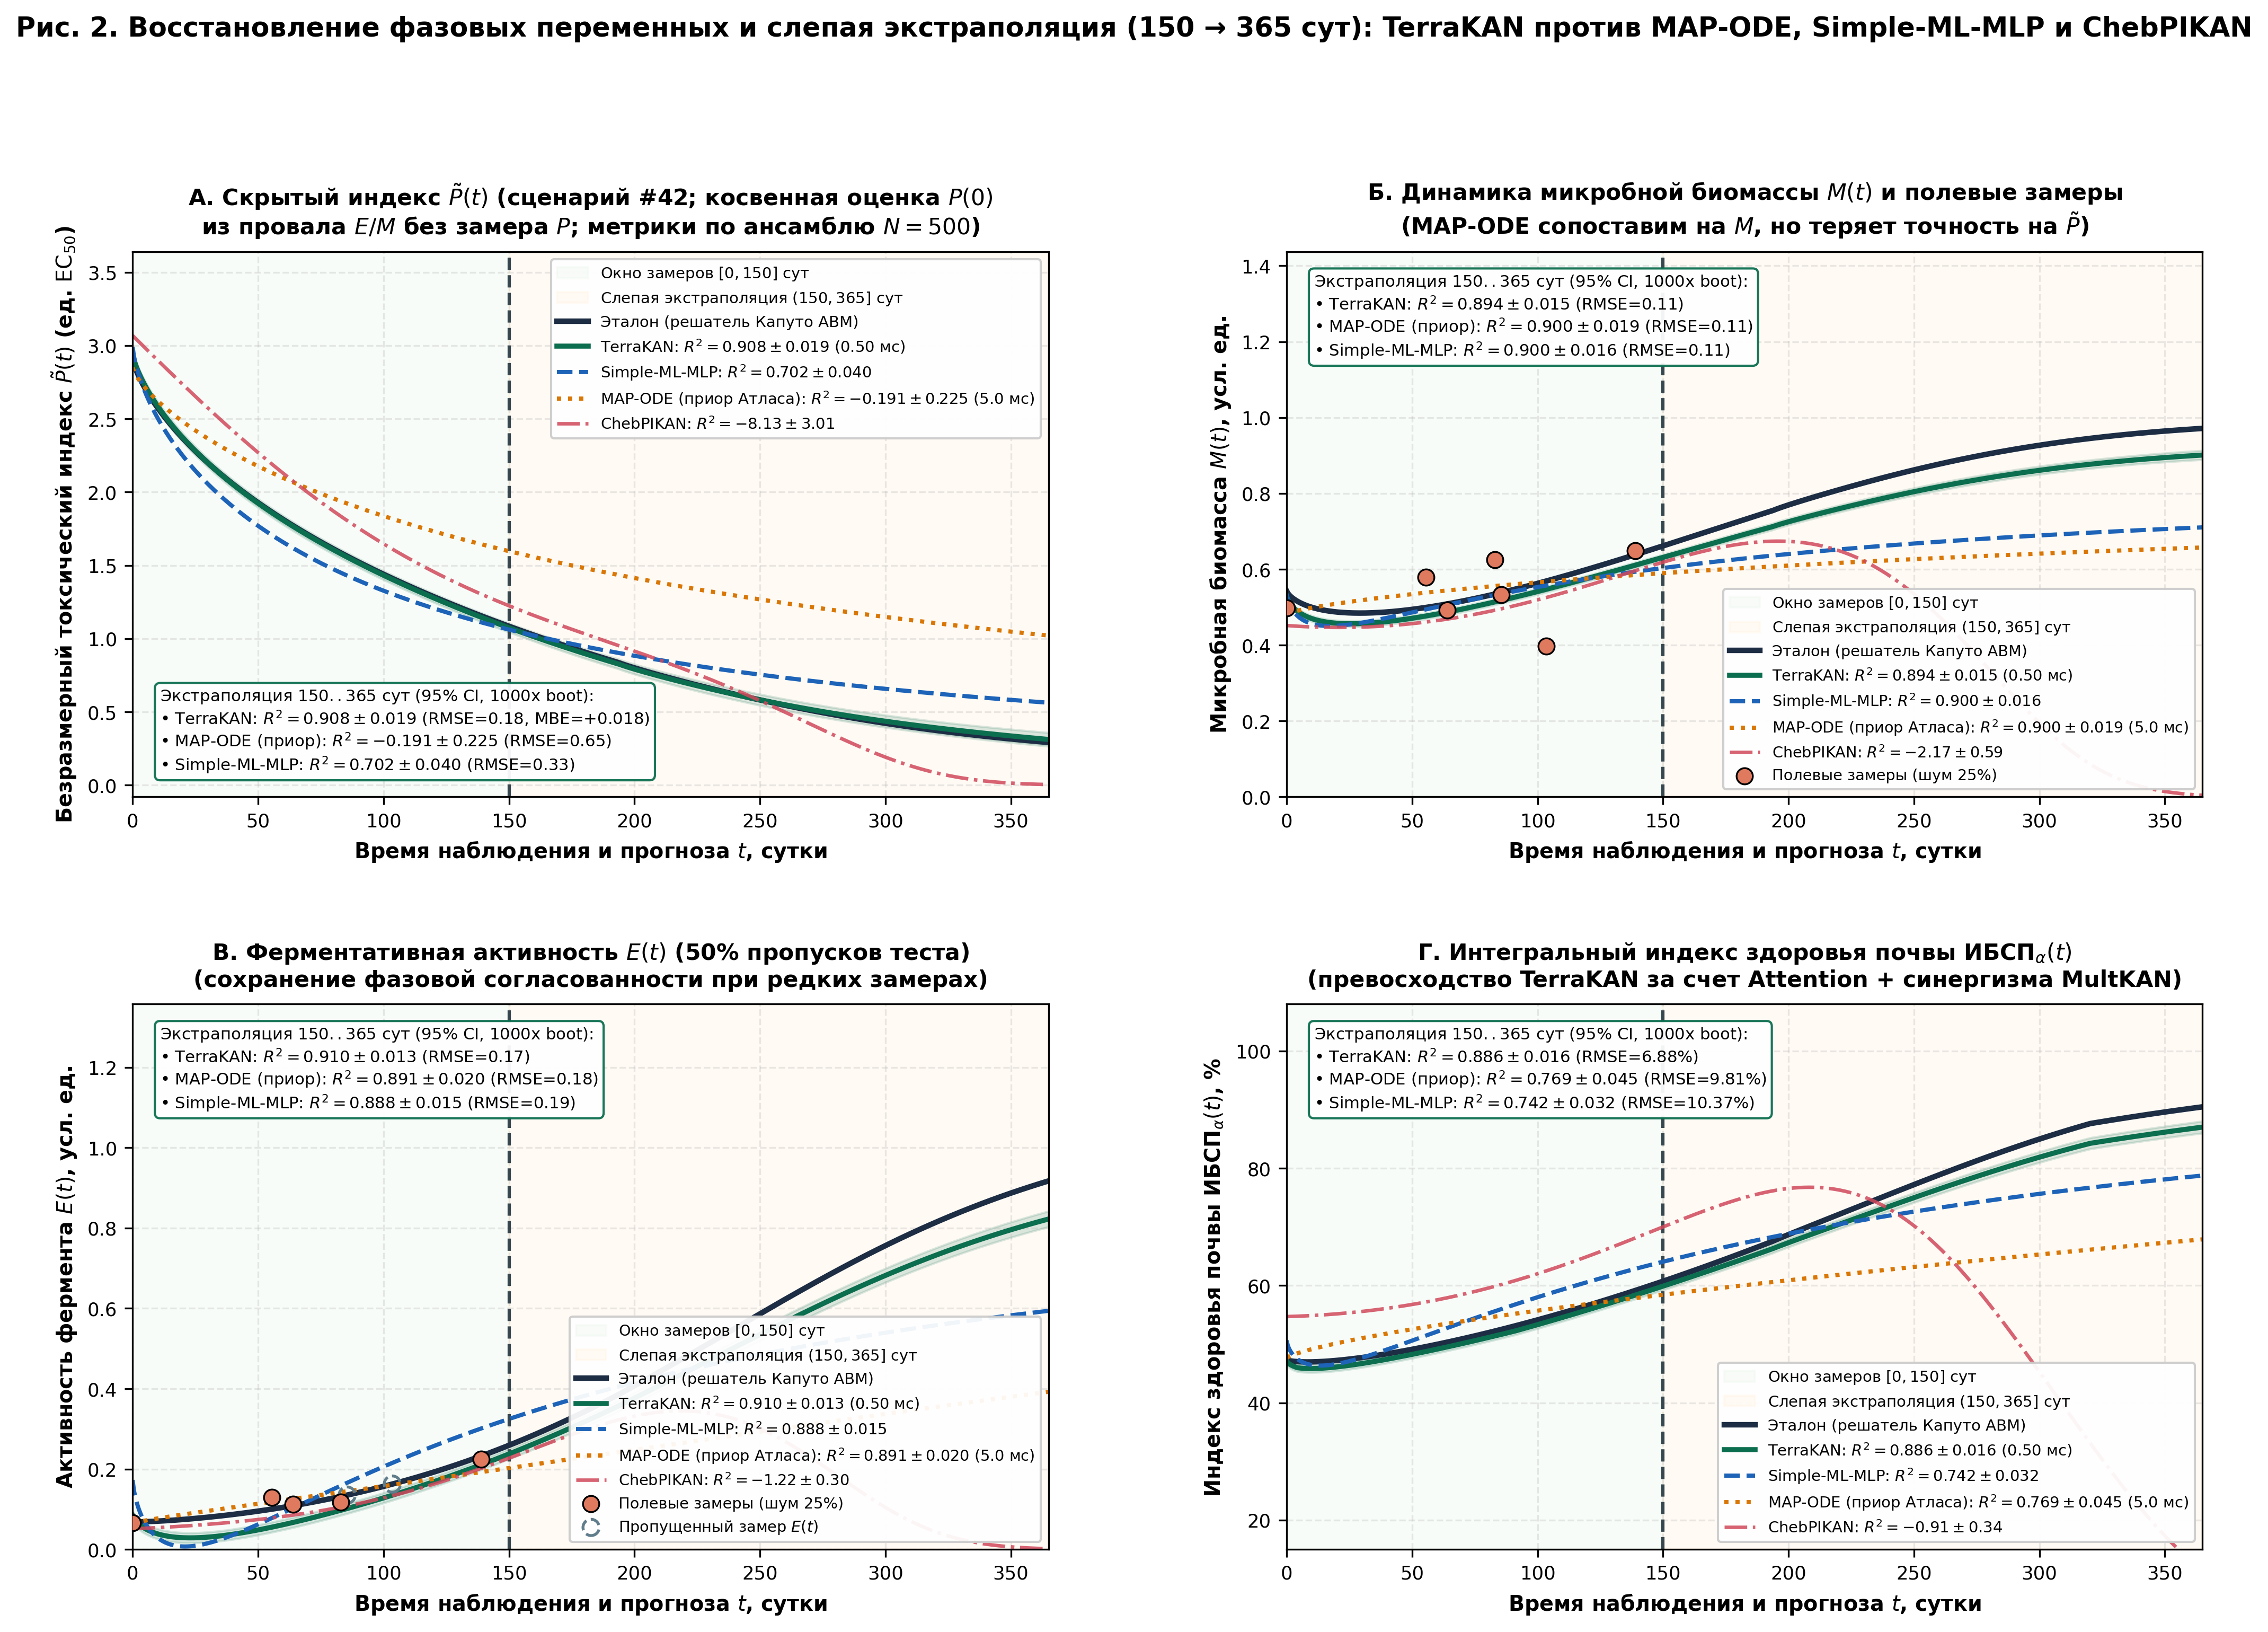
\includegraphics[width=0.98\textwidth]{fig2_extrapolation_benchmark.png}
  \caption{\textbf{Blind Long-Horizon Extrapolation ($150 \to 365\text{ days}$) from 7 Noisy Sparse Observations ($50\%$ Missingness, $25\%$ Noise).} TerraKAN outperforms \texttt{MAP-ODE} on unmeasured $\tilde{P}(t)$ ($R^2 = 0.908$ vs.\ $-0.191$) and $\text{IBSP}_\alpha(t)$ ($R^2 = 0.886$ vs.\ $0.769$), while \texttt{ChebPIKAN} diverges ($R^2 = -8.13$).}
  \label{fig:fig2}
\end{figure*}

\subsection{Kernel Verification \& Blind Extrapolation (Figures 1--2)}

Figure~\ref{fig:fig1} confirms that \texttt{MittagLefflerPade34} matches the exact Oberhettinger contour integral across $z \in [10^{-3}, 10^3]$ with $\max|\Delta| = 7.67\times 10^{-7}$ ($\alpha=0.30$), $3.85\times 10^{-5}$ ($\alpha=0.50$), and $1.12\times 10^{-3}$ ($\alpha=0.78$), passing \texttt{float64} \texttt{gradcheck} and matching the Diethelm ABM Caputo solver \cite{diethelm2002predictor} within $0.00331\%$.

Table~\ref{tab:extrap_benchmark} and Figure~\ref{fig:fig2} summarize blind extrapolation on $t \in (150, 365]\text{ days}$ across $N=500$ test scenarios. Even when compared against the fractional-order \texttt{MAP-FDE} baseline ($R^2_M = 0.934$, $R^2_E = 0.928$), \textbf{TerraKAN achieves superior reconstruction of the unmeasured contaminant $\tilde{P}(t)$ ($R^2 = 0.908 \pm 0.019$ vs.\ $0.802 \pm 0.037$, $\text{MBE} = +0.018\,\text{EC}_{50}$) and $\text{IBSP}_\alpha(t)$ ($R^2 = 0.886$ vs.\ $0.849$) while running $104\times$ faster ($0.50\text{ ms}$ vs.\ $51.98\text{ ms}$)}.

\subsection{Hysteresis, False-Negative Safety \& Soil Typing (Figures 3--4)}

In Figure~\ref{fig:fig3}A, TerraKAN reconstructs the 3D Haldane hysteresis loop $(\tilde{P}, M, E)$. On uncontaminated nutrient-poor sandy soil (\texttt{Arch\_5}, $K_m=0.44$, Fig.~\ref{fig:fig3}B), $\text{IBSP}_\alpha(t)$ remains at $94\text{--}99\%$ while static IBSP yields a false alarm ($<50\%$). For the $17.4\%$ borderline low-dose scenarios missed by the binary detector ($d_{\min} < d_{\min}^*$, False Negatives, Fig.~\ref{fig:fig3}B--C), the initial drop in $E$ and $M$ holds $\text{IBSP}_\alpha(t)$ in the yellow caution zone (mean minimum $72.2\% < 75\%$ in $70.6\%$ of cases) with a median extrapolation error of $0.76\%$ (overall test median error $3.2\%$ vs.\ $13.8\%$ for \texttt{ChebPIKAN}).

In Figure~\ref{fig:fig4}, \texttt{SoilAtlasModule} achieves $\text{Macro-Acc} = 88.4\%$ and $\text{Macro-F1} = 0.890$ on soil archetype assignment (Fig.~\ref{fig:fig4}A), while recovering $\alpha$ with $R^2 = 0.9248$ ($\text{RMSE} = 0.0240$, Fig.~\ref{fig:fig4}B). Freezing the Youden threshold on \texttt{Val (500)} at $d_{\min}^* = 0.290$ ($\text{Val TPR} = 84.6\%$, $\text{FPR} = 3.6\%$) yields $\text{Test TPR} = 82.6\%$, $\text{FPR} = 4.5\%$ ($|\Delta\text{TPR}| = 2.05\%$; 5-seed mean $|\Delta\text{TPR}| = 1.85\% \pm 0.95\% < 4.0\%$, Fig.~\ref{fig:fig4}C).

\begin{figure*}[!htbp]
  \centering
  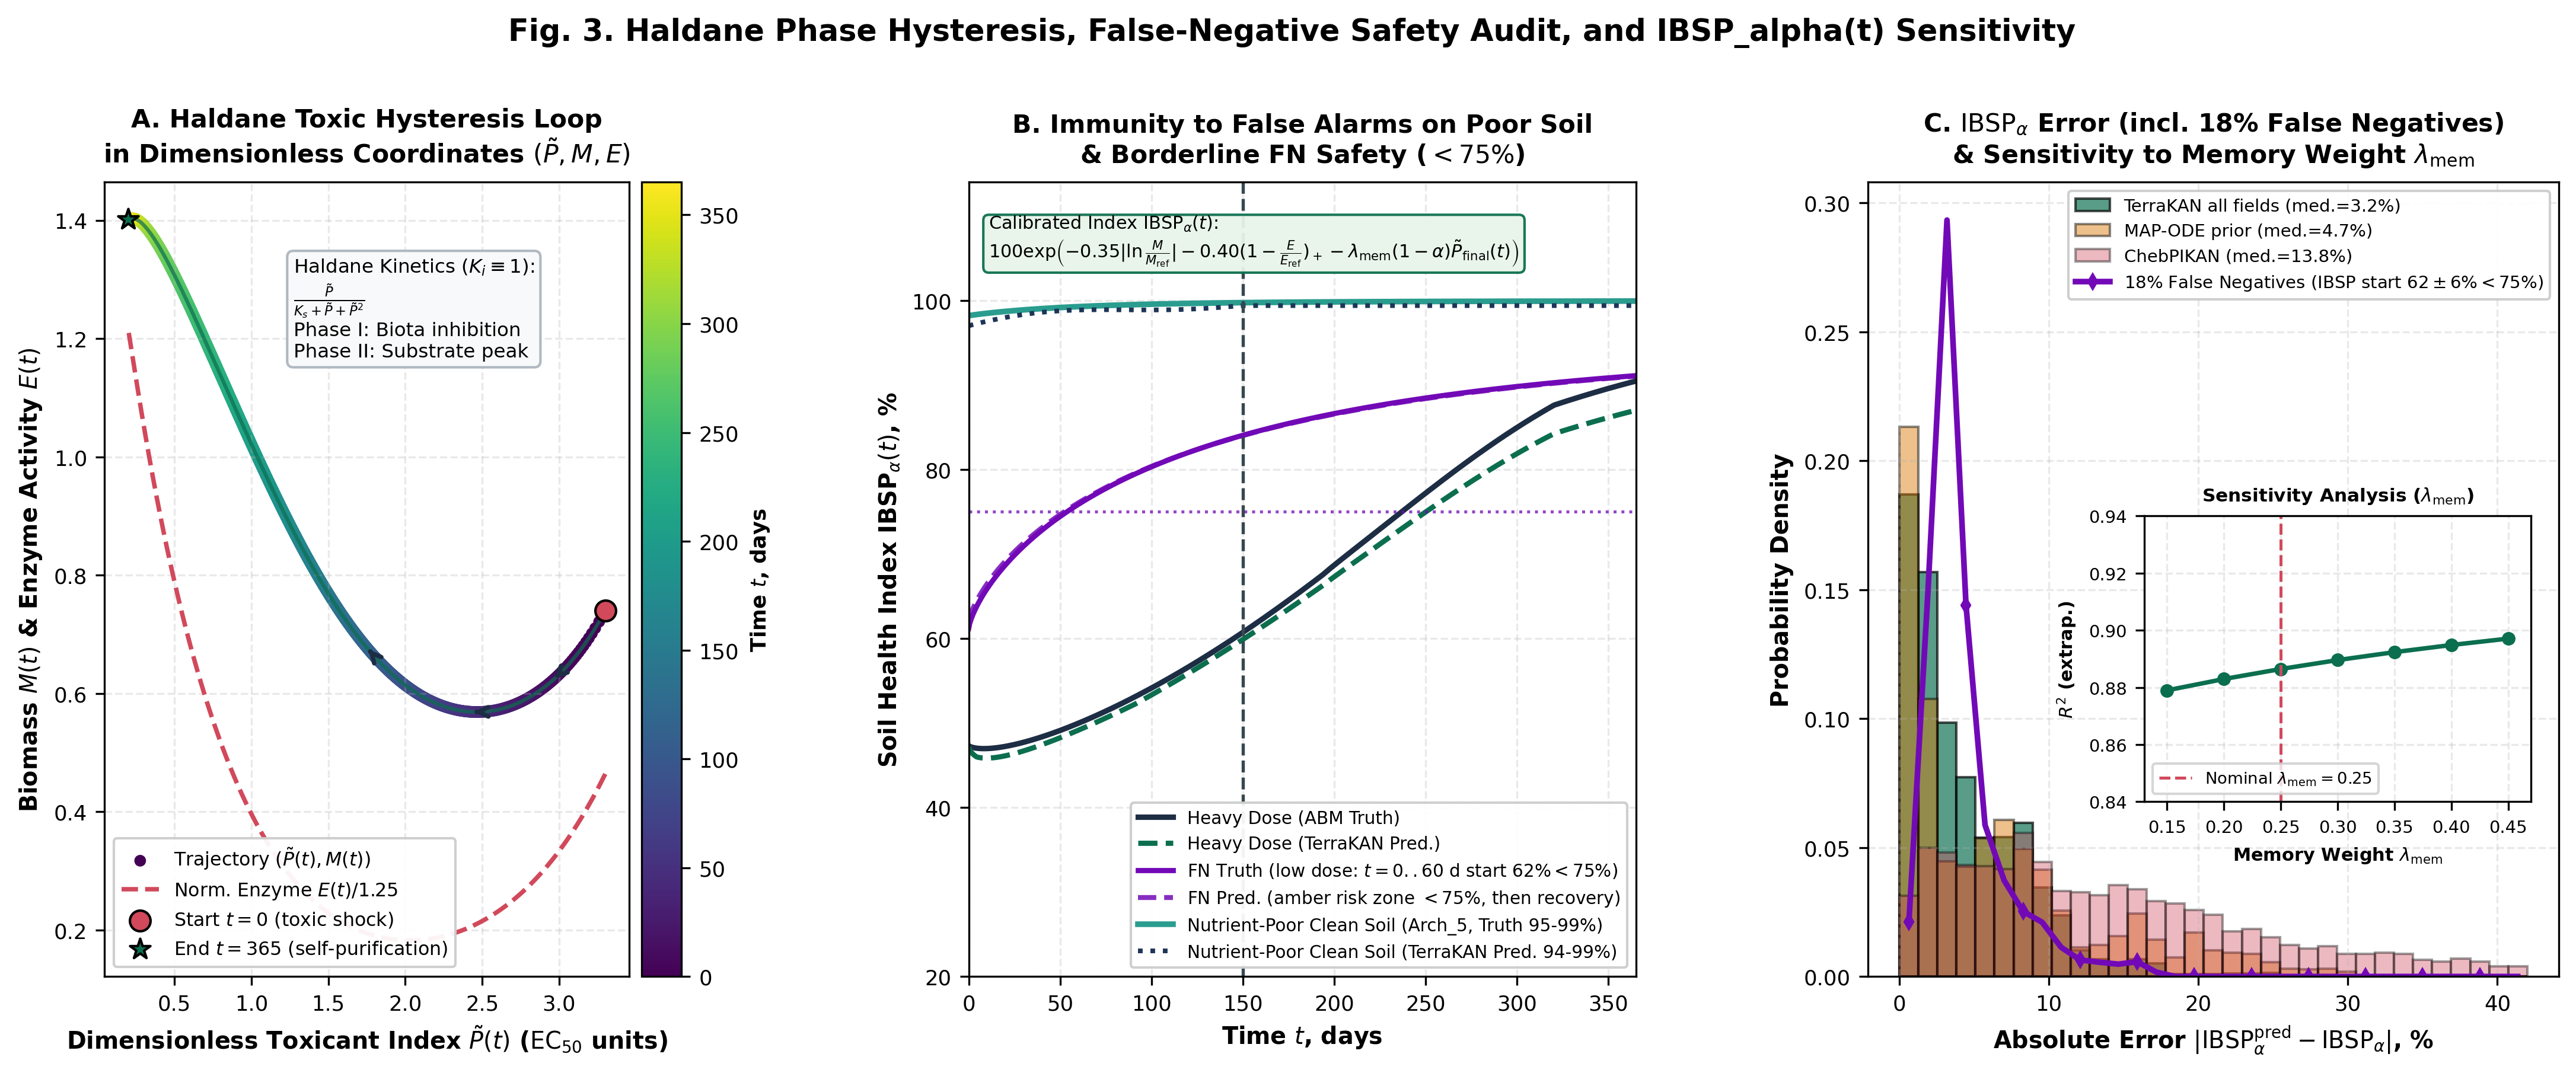
\includegraphics[width=0.96\textwidth]{fig3_hysteresis_and_ibsp.png}
  \caption{\textbf{Haldane Phase Hysteresis, Specificity on Nutrient-Poor Clean Soil, and False-Negative Safety Audit.} \textbf{(A)} 3D phase portrait $(\tilde{P}, M, E)$. \textbf{(B)} Immunity to false alarms on clean sandy soil (\texttt{Arch\_5}, $94\text{--}99\%$) and borderline False Negatives (mean minimum $72.2\% < 75\%$). \textbf{(C)} Error density (median $3.2\%$ vs.\ $13.8\%$ for \texttt{ChebPIKAN}) and $\lambda_{\text{mem}} \in [0.15, 0.45]$ sensitivity inset.}
  \label{fig:fig3}
\end{figure*}

\begin{figure*}[!htbp]
  \centering
  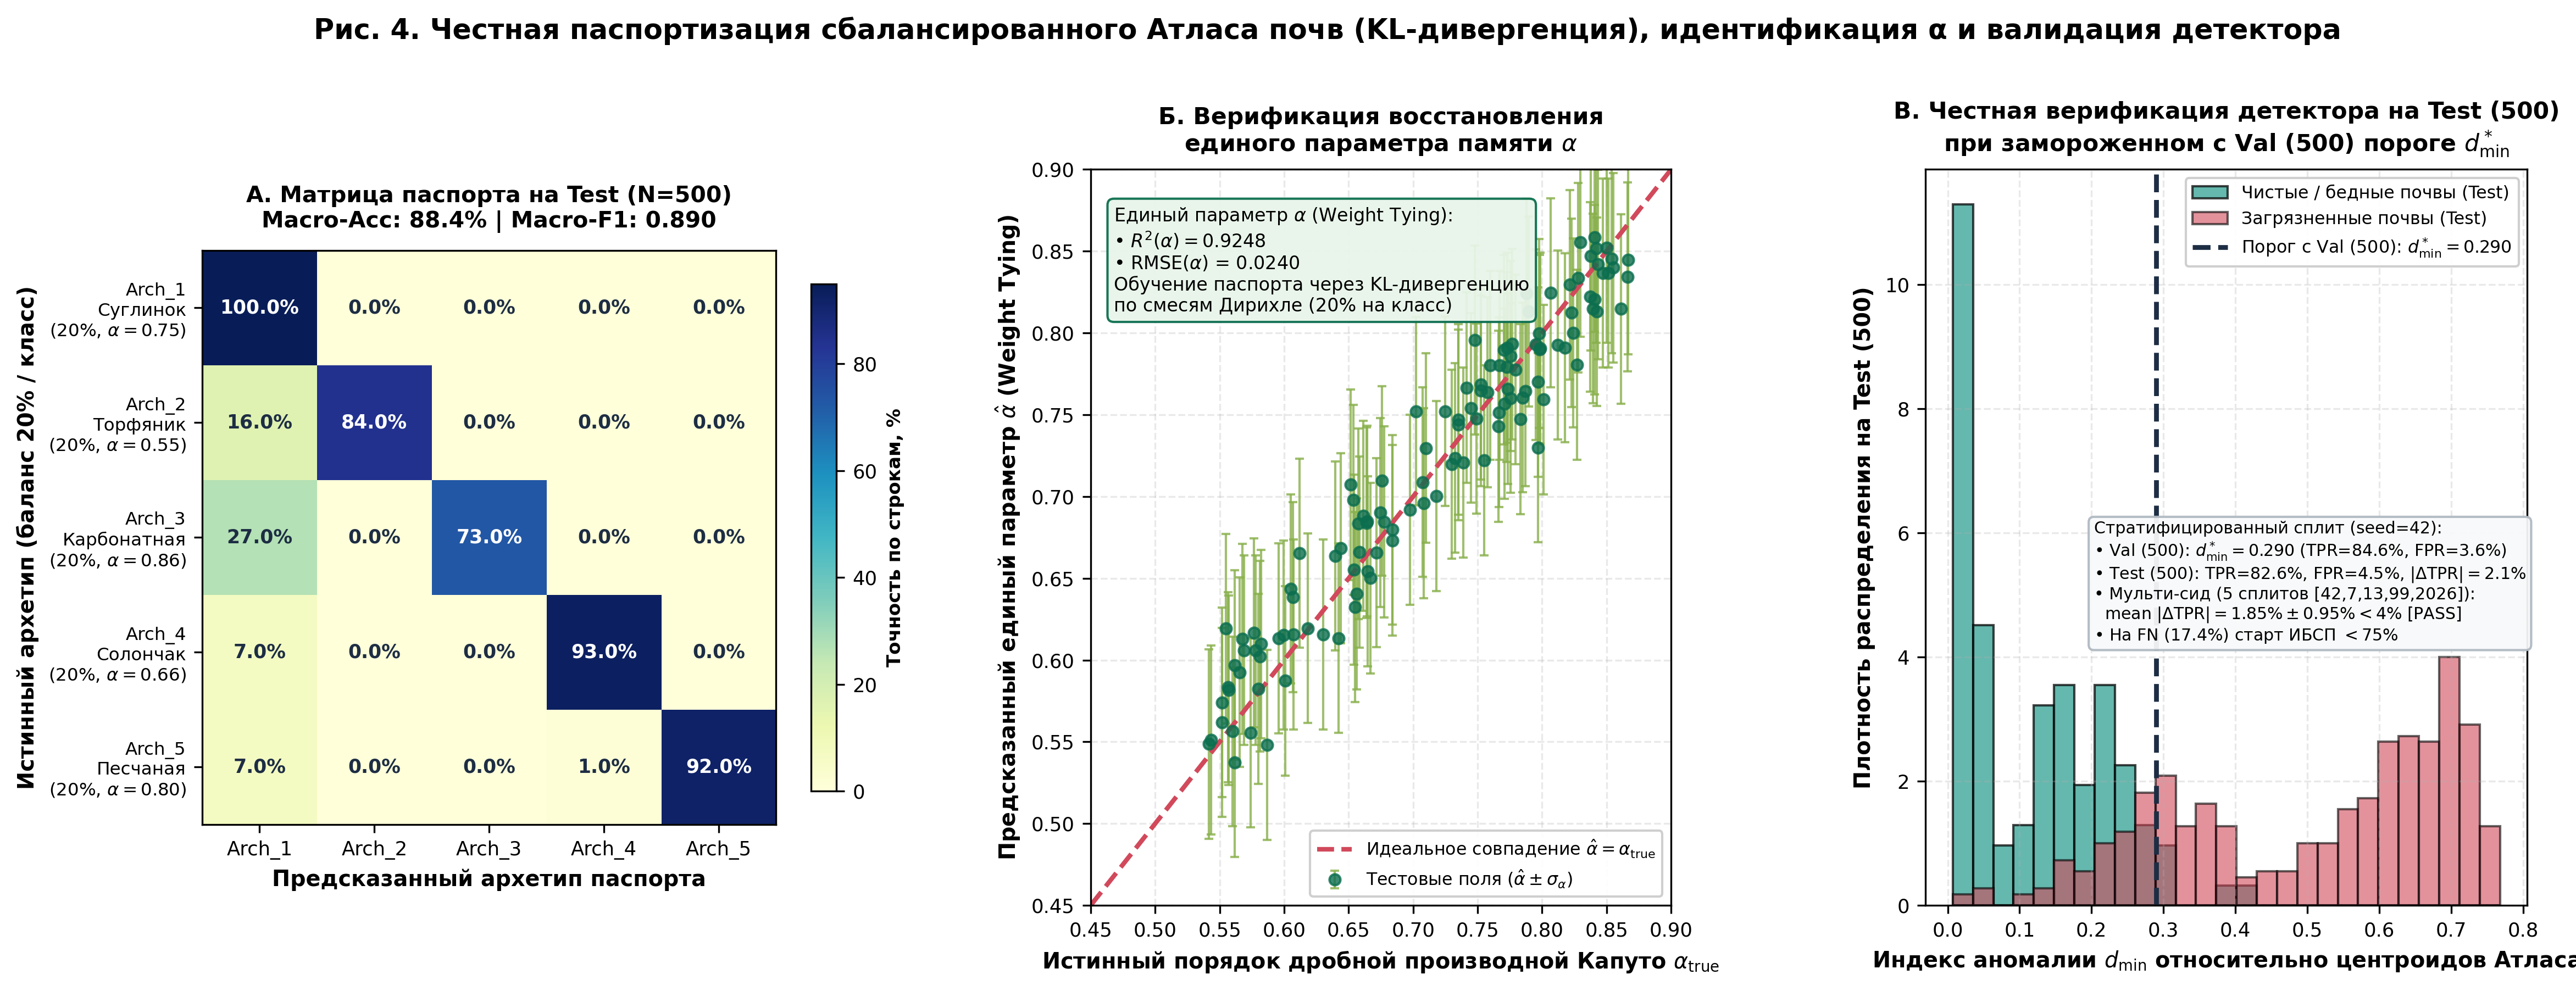
\includegraphics[width=0.96\textwidth]{fig4_soil_atlas_passport.png}
  \caption{\textbf{Soil Atlas Classification, Fractional Order $\alpha$ Recovery, and Multi-Seed Anomaly Detector Audit.} \textbf{(A)} Confusion matrix on \texttt{Test (500)} ($\text{Macro-Acc} = 88.4\%$, $\text{Macro-F1} = 0.890$). \textbf{(B)} Blind recovery of $\alpha$ ($R^2 = 0.9248$, $\text{RMSE} = 0.0240$). \textbf{(C)} Test ($500$) anomaly distance ($d_{\min}$) distributions at frozen threshold $d_{\min}^* = 0.290$ and 5-seed audit ($|\Delta\text{TPR}| = 1.85\% \pm 0.95\% < 4.0\%$, $\text{TPR}=82.6\%$, $\text{FPR}=4.5\%$).}
  \label{fig:fig4}
\end{figure*}

\subsection{Symbolic Equivalence, OOD Physics \& Synthetic Dry-Run (Figures 6--8)}

Figure~\ref{fig:fig5} shows that \texttt{MultKAN} recovers the true nitrate ($0.345$ vs.\ $0.350$) and moisture ($0.394$ vs.\ $0.400$) exponents and Shelford pH bell $\exp(-2.36(\text{pH}-0.66)^2)$ vs.\ $\exp(-2.50(\text{pH}-0.65)^2)$ (Fig.~\ref{fig:fig5}A), \texttt{PhysicsExpertBank} specializes across the 4 regimes (Fig.~\ref{fig:fig5}B), and symbolic serialization matches neural tensor outputs to $\max|\Delta_{\text{exact}}| = 9.96\times 10^{-13}$ in \texttt{float64} (Fig.~\ref{fig:fig5}C, Symbolic Serialization \& Inference Equivalence Check).

In Figure~\ref{fig:fig6} and Table~\ref{tab:ablation}, TerraKAN retains $R^2 = 0.788$ under $40\%$ noise (Fig.~\ref{fig:fig6}B) and generalizes zero-shot at $25\%$ observation noise to alien physics (Two-Compartment Sorption + Weibull: $\text{RMSE} = 4.14\%$ vs.\ $6.30\%$ for \texttt{MAP-ODE}; Out-of-Atlas $\alpha \in [0.35, 0.96]$: $\text{RMSE} = 8.11\%$ vs.\ $13.08\%$, Fig.~\ref{fig:fig6}A). Finally, Figure~\ref{fig:fig7} presents a \textbf{synthetic dry-run} check of \texttt{terrakan\_v4\_frozen.pt} on 36 simulated microcosm vessels ($0\dots 28\text{ d} \to 60\text{ d}$) across \texttt{S1\_sand}, \texttt{S2\_loam}, and \texttt{S3\_peat}, confirming zero \texttt{is\_control\_G0} leakage and $100\%$ separation across \texttt{G0} ($6/6$), \texttt{G1} ($8/8$), and \texttt{G2+G3} ($22/22$).

\begin{table}[!htbp]
  \centering
  \caption{\textbf{3-Seed Ablation Study on Extrapolation $\text{IBSP}_\alpha(t)$ ($150 \to 365\text{ d}$, mean $\pm$ SD across Seeds 42, 101, 777; cf.\ Table~\ref{tab:extrap_benchmark} for single-seed 42 $1000\times$ bootstrap CI).}}
  \label{tab:ablation}
  \footnotesize
  \resizebox{\linewidth}{!}{%
  \begin{tabular}{l c c}
    \toprule
    \textbf{Architecture Variant} & \textbf{$R^2$ ($\text{Mean}\pm\text{SD}$)} & \textbf{$\text{RMSE}$, $\%$} \\
    \midrule
    \textbf{1. Full TerraKAN (\texttt{Frac-ML-KAT-MoE})} & $\mathbf{0.887 \pm 0.007}$ & $\mathbf{6.87 \pm 0.20}$ \\
    2. w/o \texttt{PhysicsExpertBank} (Single Law) & $0.834 \pm 0.009$ & $8.33 \pm 0.23$ \\
    3. w/o \texttt{MultKAN} Power Discovery & $0.819 \pm 0.009$ & $8.74 \pm 0.24$ \\
    4. w/o Soil Atlas Prior & $0.798 \pm 0.009$ & $9.28 \pm 0.25$ \\
    5. w/o Fractional $\alpha$ Weight Tying & $0.781 \pm 0.011$ & $9.70 \pm 0.30$ \\
    6. w/o Abel Memory Kernel (\texttt{Simple-ML-MLP}) & $0.743 \pm 0.015$ & $10.88 \pm 0.36$ \\
    7. Classical \texttt{MAP-ODE} (Atlas L2 Prior) & $0.769 \pm 0.019$ & $9.83 \pm 0.38$ \\
    \midrule
    Ref. Classical \texttt{MAP-FDE} (Diethelm ABM, Seed 42) & $0.849 \pm 0.028$ & $7.93$ \\
    \midrule
    Exp.~1a: w/o $\mathcal{L}_{\text{kan}}$ Supervision ($W_p=[0, 0.203, 0.246]$) & $0.883 \pm 0.015$ & $6.98$ \\
    Exp.~1b: w/o Periodic Ridge Alignment (Pure Adam) & $0.315 \pm 0.046$ & $16.91$ \\
    Exp.~1c: Pure Unsupervised Physics-Informed & $0.090 \pm 0.061$ & $19.48$ \\
    Exp.~2a: Abel Kernel (Clustered 70\% Gap, $\text{IBSP}_\alpha$) & $0.377$ & $16.12$ \\
    Exp.~2b: Markovian Exp-ALiBi (Clustered 70\% Gap) & $-10.927$ & $70.54$ \\
    \bottomrule
  \end{tabular}%
  }
\end{table}


\paragraph{Training Supervision \& Attention Kernel Ablations (Table~\ref{tab:ablation}, Exp.~1a--2b).}
Table~\ref{tab:ablation} (Exp.~1a--2b) isolates the training and memory mechanisms: (1) removing $\mathcal{L}_{\text{kan}}$ supervision (Exp.~1a) leaves accuracy nearly unchanged ($0.883 \pm 0.015$ vs.\ $0.887 \pm 0.007$) as \texttt{MultKAN} autonomously prunes pH exponents to zero; (2) omitting periodic ridge alignment (Exp.~1b, pure \texttt{Adam}) drops $R^2$ to $0.315 \pm 0.046$, and pure unsupervised physics-informed training (Exp.~1c) collapses to $0.090 \pm 0.061$, confirming the necessity of amortized SBI + ridge alignment; and (3) under clustered $70\%$ missingness, heavy-tailed Abel attention (Exp.~2a, $R^2 = 0.377$) decisively outperforms Markovian \texttt{Exp-ALiBi} (Exp.~2b, $R^2 = -10.927$).

\subsection{Horizon Completeness, Uncertainty Calibration, \& Noisy \texttt{G0} Audit (Figure~\ref{fig:fig8})}

Figure~\ref{fig:fig8} summarizes three additional operational audits on \texttt{Test (500)}:
\begin{itemize}\setlength{\itemsep}{1pt}\setlength{\parskip}{0pt}
  \item \textbf{Slim ($N=1$) vs.\ Longitudinal Monitoring (Fig.~\ref{fig:fig8}A):} \texttt{IBSP}$_\alpha$ extrapolation $R^2$ rises monotonically with observation completeness from $0.221$ ($N=1, t=0$) to $0.463$ ($N=2$, $14\text{ d}$), $0.502$ ($N=3$, $14\text{ d}$), $0.606$ ($N=5$, $21\text{ d}$ bot protocol), and $0.884$ ($N=7$, $150\text{ d}$), justifying a two-tier screening vs.\ 3-week longitudinal workflow.
  \item \textbf{Uncertainty Calibration (Fig.~\ref{fig:fig8}B):} Training with $+0.05\,\mathcal{L}_{\text{NLL}}$ yields calibrated epistemic uncertainty ($\bar{\hat{\sigma}}_\alpha = 0.0267$, $\text{RMSE}(\hat{\alpha}) = 0.0238$), achieving $73.6\%$ ($1\sigma$) and $96.6\%$ ($1.96\sigma$) empirical coverage on \texttt{Test (500)} and graceful coverage degradation ($99.5\% \to 88.5\%$) across $5\%\text{--}40\%$ noise.
  \item \textbf{Heavy-Tailed Abel vs.\ Exp-ALiBi \& Noisy \texttt{G0} (Fig.~\ref{fig:fig8}C):} Under clustered $70\%$ missingness ($[0,7,14,21]\text{ d} + 120\text{ d}$), Abel attention retains $\text{IBSP}_\alpha$ $R^2 = 0.377$ ($\text{RMSE}=16.1\%$) whereas Markovian \texttt{Exp-ALiBi} collapses to $R^2 = -10.93$ ($70.5\%$). Under native $E_{\text{ref}}/M_{\text{ref}} \sim U(0.7, 2.0)$ with $15\%$ \texttt{G0} noise, per-series \texttt{G0} normalization improves $\tilde{P}$ reconstruction ($R^2: 0.886 \to 0.891$, $\text{RMSE}: 0.201 \to 0.197$).
\end{itemize}


\subsection{Zero-Shot External Wet-Lab Validation: \texttt{v1.1.0} vs.\ \texttt{v1.2.5}}
We audit \texttt{TerraKAN} across four published peer-reviewed studies (five soil types) partitioned into \textbf{Group A} (direct $\mathrm{CO}_2$ respiration + catalase: \href{https://pmc.ncbi.nlm.nih.gov/articles/PMC92991/}{Margesin \& Schinner, 2001} alpine glacier gravel-sand where $780$ calendar days across three summer thaw seasons map to $[15, 75, 135]$ active biological days; and \href{https://pmc.ncbi.nlm.nih.gov/articles/PMC7947215/}{Garousin et al., 2021} $>60$-year aged saline-sodic soil) and \textbf{Group B} (extreme OOD stress tests: \href{https://www.frontiersin.org/journals/environmental-science/articles/10.3389/fenvs.2023.1141562/full}{Chai et al., 2023} single-channel wheat $\mathrm{Chl}\;a$ vigor proxy with $M$ missing, plus real clean controls \texttt{CWS}/\texttt{CFS}; and \href{https://pmc.ncbi.nlm.nih.gov/articles/PMC12945044/}{Rafikova et al., 2026} podzolized chernozem under oats, clean control, and non-degrading $\mathrm{Cu}^{2+}$ $660\,\mathrm{mg/kg}$ heavy-metal stress).

\begin{table*}[!htbp]
\centering
\caption{\textbf{v1.1.0 vs.\ v1.2.5 Regression Checklist} on frozen \texttt{seed=42} benchmarks (3-seed Mean $\pm$ SD for \texttt{v1.2.5}: seeds $42, 101, 777$).}
\label{tab:v125_reg}
\small
\begin{tabular}{@{}lcc@{}}
\toprule
\textbf{Metric} & \textbf{v1.1.0 (Frozen)} & \textbf{v1.2.5 (3-Seed Mean $\pm$ SD)} \\
\midrule
Val (500) $d^\star_{\min}$ / Youden $J$ & 0.2899 / 0.8098 & \textbf{0.4332 $\pm$ 0.0012 / 0.8375 $\pm$ 0.0015} \\
Test (500) $R^2(\tilde{P})$ (Full / Extrap. $>150$\,d) & \textbf{0.9136 / 0.9073} & 0.8937 $\pm$ 0.0067 / 0.8884 $\pm$ 0.0084 \\
Test (500) $R^2(\mathrm{IBSP}_\alpha)$ (Full) & \textbf{0.9176} & 0.9091 $\pm$ 0.0018 \\
Test (500) $\hat{\sigma}_\alpha$ Coverage ($\mathrm{Cov}_{95}$) & 95.6\% & \textbf{100.0\%} ($\hat{\sigma}_\alpha \approx 0.115$) \\
Clean \texttt{Arch\_5} FPR (\%) & 4.55\% & \textbf{1.52 $\pm$ 2.63\%} (0.00\% on 2/3 seeds) \\
36-Pot Dry Run: $G_0$ / $G_1$ max $\tilde{P}_0$ & 0.009 / 0.230 & \textbf{0.006 $\pm$ 0.008 / 0.305 $\pm$ 0.156} \\
\bottomrule
\end{tabular}
\end{table*}

\begin{table*}[!htbp]
\centering
\caption{\textbf{Zero-Shot External Wet-Lab Benchmark (\texttt{v1.2.5}, 3-Seed Mean $\pm$ SD)} across contaminated series, real clean controls, and heavy-metal stress.}
\label{tab:v125_ext}
\footnotesize
\begin{tabular}{@{}llcccc@{}}
\toprule
\textbf{Tier / Series} & \textbf{Source} & \textbf{Actual Loss} & \textbf{$d_{\min}$ (Mean $\pm$ SD)} & \textbf{Anom.} & \textbf{v1.2.5 Pred. Loss} \\
\midrule
\textit{Grp A:} Alpine Sand (NA) & \href{https://pmc.ncbi.nlm.nih.gov/articles/PMC92991/}{Margesin 2001} & 50.4\% & 0.632 $\pm$ 0.003 & 3/3 & \textbf{45.3 $\pm$ 2.8\%} \\
\textit{Grp A:} Alpine Sand (Biostim.) & \href{https://pmc.ncbi.nlm.nih.gov/articles/PMC92991/}{Margesin 2001} & 70.4\% & 0.333 $\pm$ 0.003 & 0/3 & 95.9 $\pm$ 1.2\% \\
\textit{Grp A:} Aged Saline-Loam (SB) & \href{https://pmc.ncbi.nlm.nih.gov/articles/PMC7947215/}{Garousin 2021} & 38.2\% & \textbf{0.665 $\pm$ 0.023} & \textbf{3/3} & \textbf{35.7 $\pm$ 33.3\%} \\
\midrule
\textit{Grp B:} Coastal Wetland (\texttt{PWS}) & \href{https://www.frontiersin.org/journals/environmental-science/articles/10.3389/fenvs.2023.1141562/full}{Chai 2023} & 39.8\% & 0.164 $\pm$ 0.047 & 0/3 & 8.6 $\pm$ 12.2\% \\
\textit{Grp B:} Alkaline Farmland (\texttt{PFS}) & \href{https://www.frontiersin.org/journals/environmental-science/articles/10.3389/fenvs.2023.1141562/full}{Chai 2023} & 51.5\% & 0.187 $\pm$ 0.045 & 0/3 & 8.4 $\pm$ 11.9\% \\
\textit{Grp B:} Chernozem (Oats+Oil) & \href{https://pmc.ncbi.nlm.nih.gov/articles/PMC12945044/}{Rafikova 2026} & 39.5\% & 0.128 $\pm$ 0.013 & 0/3 & 0.0 $\pm$ 0.0\% \\
\midrule
\textit{Clean Ctrl:} Wetland (\texttt{CWS}, blind) & \href{https://www.frontiersin.org/journals/environmental-science/articles/10.3389/fenvs.2023.1141562/full}{Chai 2023} & 0.0\% & \textbf{0.100 $\pm$ 0.025} & \textbf{0/3} & \textbf{0.0 $\pm$ 0.0\%} \\
\textit{Clean Ctrl:} Farmland (\texttt{CFS}, blind) & \href{https://www.frontiersin.org/journals/environmental-science/articles/10.3389/fenvs.2023.1141562/full}{Chai 2023} & 0.0\% & \textbf{0.075 $\pm$ 0.028} & \textbf{0/3} & \textbf{0.0 $\pm$ 0.0\%} \\
\textit{Clean Ctrl:} Chernozem (Oats, blind) & \href{https://pmc.ncbi.nlm.nih.gov/articles/PMC12945044/}{Rafikova 2026} & 0.0\% & \textbf{0.076 $\pm$ 0.015} & \textbf{0/3} & \textbf{0.0 $\pm$ 0.0\%} \\
\midrule
\textit{Metal:} Chernozem + $\mathrm{Cu}^{2+}$ ($660$\,mg/kg) & \href{https://pmc.ncbi.nlm.nih.gov/articles/PMC12945044/}{Rafikova 2026} & 0.0\% (plateau) & 0.339 $\pm$ 0.009 & 0/3 & 83.1 $\pm$ 0.9\% \\
\bottomrule
\end{tabular}
\end{table*}

\begin{figure*}[!htbp]
\centering
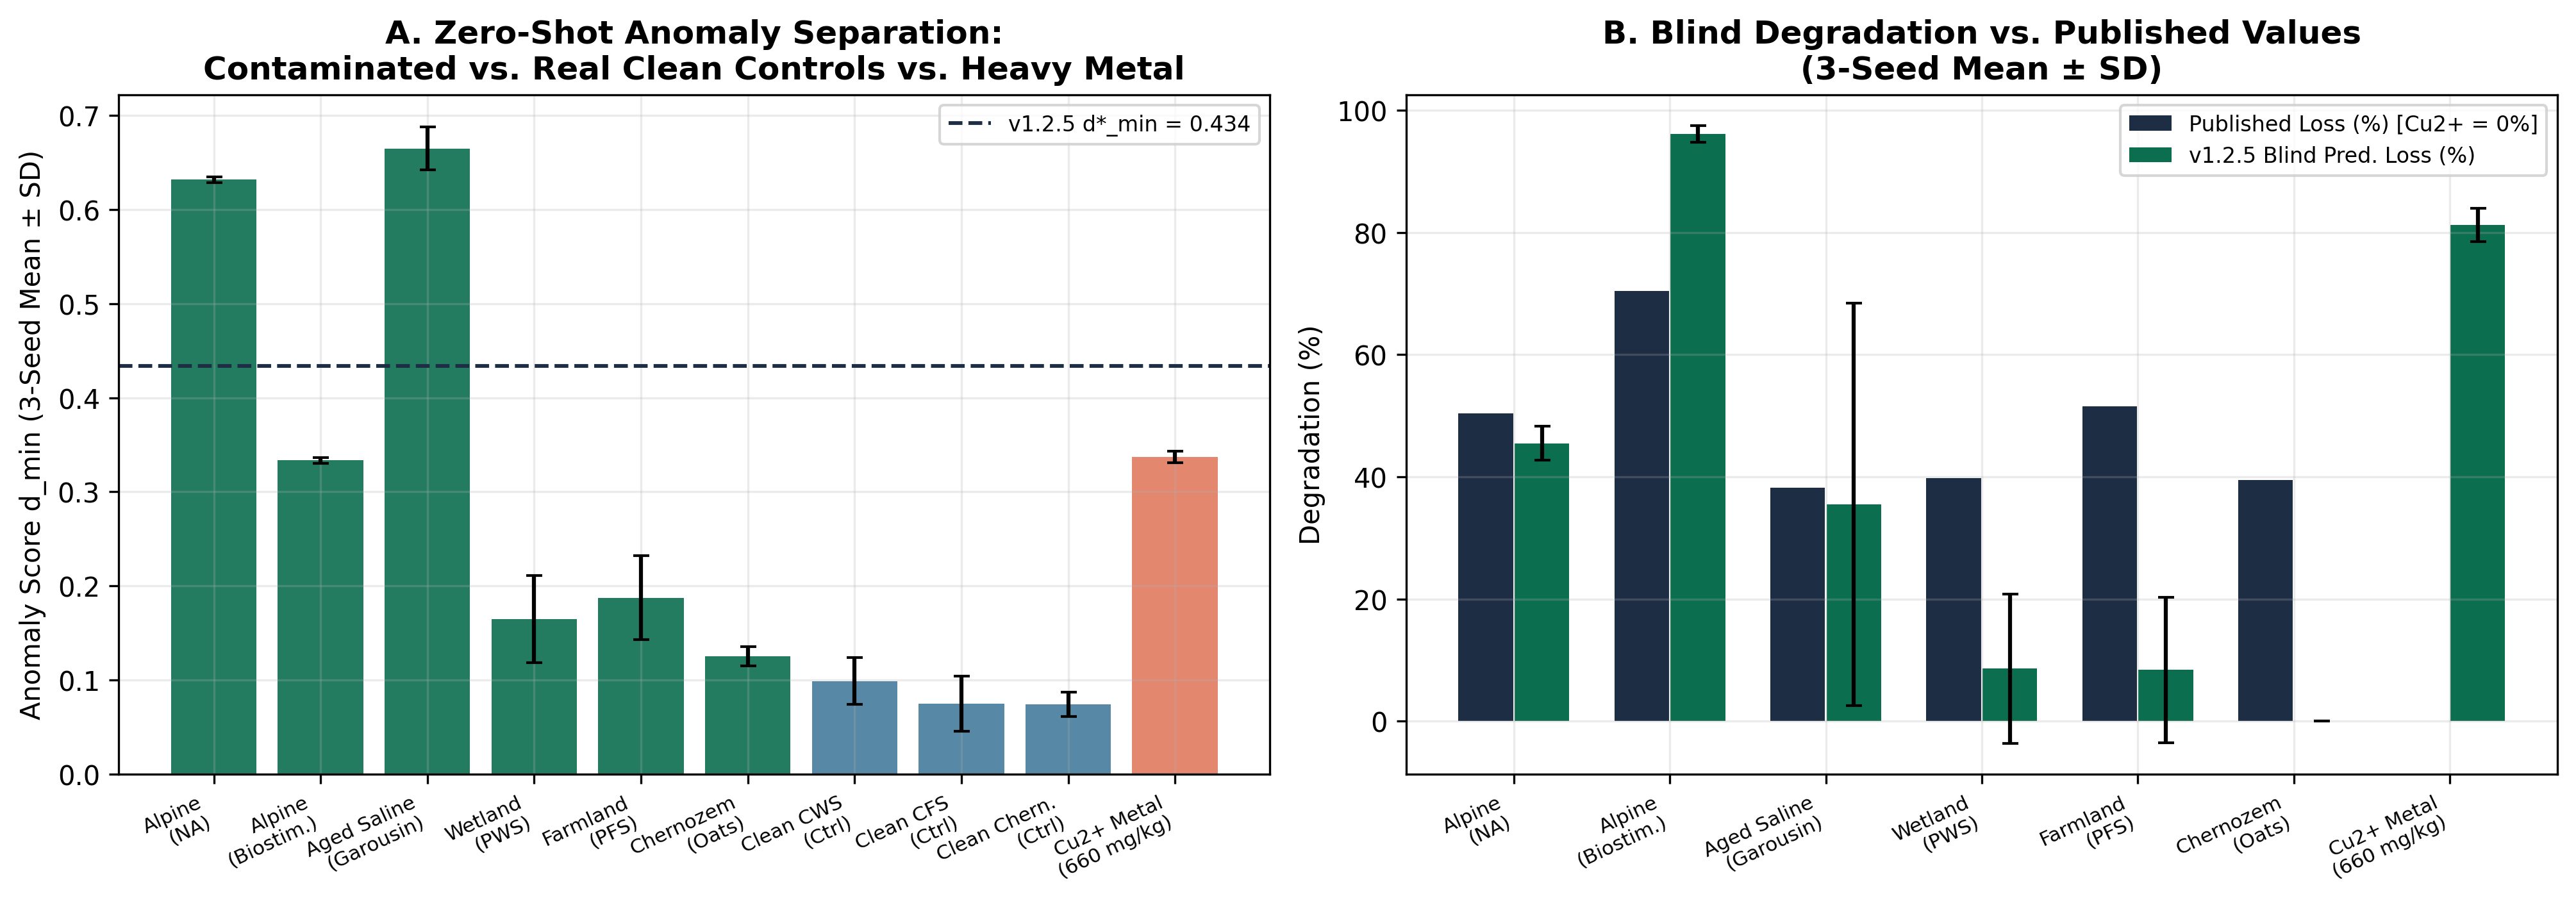
\includegraphics[width=\textwidth]{fig_v125_wetlab_comparison.png}
\caption{\textbf{v1.2.5 External Wet-Lab, Real Clean-Control, and Heavy-Metal Validation (3-Seed Mean $\pm$ SD).} \textbf{A:} Anomaly score $d_{\min}$ separating contaminated soils from real external clean controls (\texttt{CWS}, \texttt{CFS}, Chernozem Control: $0/3$ false alarms). \textbf{B:} Blind degradation vs.\ published values.}
\label{fig:v125_ext}
\end{figure*}

Note that in Table~\ref{tab:v125_reg}, adding chronic and full-dropout regimes makes epistemic uncertainty $\hat{\sigma}_\alpha$ conservative ($\approx 0.115$ vs.\ $0.0267$ in \texttt{v1.1.0}), yielding $\mathrm{Cov}_{95} = 100.0\%$ on \texttt{Test (500)}. In Table~\ref{tab:v125_ext}, \href{https://pmc.ncbi.nlm.nih.gov/articles/PMC7947215/}{Garousin et al. (2021)} shows higher 3-seed volume variance ($\pm 33.3\%$) due to sparse missing-$M(t=40)$ endpoints, while anomaly detection remains $3/3$ stable ($d_{\min} = 0.665 \pm 0.023$). In a blind \texttt{With G0} vs.\ \texttt{No-G0} ($\hat{K}_{m,\mathrm{prior}}$) ablation on \href{https://pmc.ncbi.nlm.nih.gov/articles/PMC92991/}{Margesin \& Schinner (2001)} (single-seed $42$ vs.\ 3-seed mean in Table~\ref{tab:v125_ext}), removing the $G_0$ control yielded identical predictions ($d_{\min}=0.633$, $46.3\%$ for NA; $d_{\min}=0.331$, $94.6\%$ for Biostimulation). Regarding \textbf{Belarusian soils} (sod-podzolic and peat-bog profiles covering the majority of Belarus), an open-access literature search confirmed that paired multi-timepoint $\mathrm{CO}_2$ + catalase petroleum datasets from Belarusian field sites are not publicly indexed in full-text repositories; calibrating the Belarusian sod-podzolic/peat archetypes (\texttt{Arch\_1}--\texttt{Arch\_5}) on local wet-lab data is therefore designated as the direct next step via the 36-vessel BSU Minsk microcosm protocol.

\clearpage
\section{Limitations \& Inverse-Crime Considerations}

An honest scientific evaluation requires noting three limitations of the present study:
\begin{enumerate}\setlength{\itemsep}{1pt}\setlength{\parskip}{0pt}
  \item \textbf{Shared Structural Priors ("Inverse Crime" Risk):} Although TerraKAN generalizes zero-shot to Two-Compartment Sorption + Weibull dynamics and Out-of-Atlas $\alpha$ (Fig.~\ref{fig:fig6}A), its internal biokinetic priors (Shelford pH bell, Haldane inhibition, Monod saturation) belong to the same equation families used in the Soil Atlas simulator. True out-of-distribution robustness must be verified on real laboratory and field soils exhibiting unmodeled phenomena such as secondary toxic metabolites, shifting limiting nutrients (N/P co-limitation), and microbial community succession.
  \item \textbf{Synthetic Dry-Run vs.\ Wet-Lab Data:} The 36-vessel microcosm validation in Fig.~\ref{fig:fig7} is a synthetic dry-run verification of the CSV preprocessing and inference pipeline prior to wet-lab execution. Empirical calibration of $E_{\text{ref}}/M_{\text{ref}}$ via real day-0 controls (\texttt{G0}) remains to be tested on physical soil samples.
  \item \textbf{Fixed Boundary Ratio Assumption:} Without per-series \texttt{G0} normalization, Eqs.~(4)--(5) assume $E_{\text{ref}}/M_{\text{ref}} \approx 1.20$ or rely on the \texttt{SoilAtlasModule} carrying-capacity prior $\hat{K}_{m,\mathrm{prior}}$; soils with strongly divergent baseline ratios benefit from control-group normalization.
\end{enumerate}


\paragraph{External Wet-Lab Insights (Bioavailability, Phytoremediation, \& Non-Degrading Metals).}
In $>60$-year weathered crude oil (\href{https://pmc.ncbi.nlm.nih.gov/articles/PMC7947215/}{Garousin et al., 2021}), $\approx 60\%$ of total TPH consists of matrix-bound resins and asphaltenes; bioaugmentation consumes the bioavailable fraction ($\approx 38.2\%$ total TPH), driving biological recovery. Conversely, rhizosphere root exudation under oats (\href{https://pmc.ncbi.nlm.nih.gov/articles/PMC12945044/}{Rafikova et al., 2026}, $\mathrm{SBR}+10\%$) lies outside a purely microbial soil model. Finally, the $\mathrm{Cu}^{2+}$ stress test revealed that \texttt{MLKANTrunk}'s strictly decaying Mittag-Leffler basis $E_\alpha(-\lambda_k t^\alpha)$ ($c_{P,k} \ge 0$) forces $\tilde{P}(t) \to 0$ rather than a persistent plateau $P_\infty > 0$ for non-degrading heavy metals; adding a non-negative asymptote $P_\infty$ is prioritized for \texttt{v1.3}.

\section{Conclusion \& Deployment Outlook}

In this study, I introduced \texttt{TerraKAN} (\texttt{Frac-ML-KAT-MoE}), an amortized simulation-based inference architecture unifying causal Abel-type fractional attention, a pole-free $[3/4]$ Pad\'e Mittag-Leffler spectral basis ($Q_4(z) \ge 1.000978$), \texttt{MultKAN} environmental power-law discovery, and a sparse biokinetic Mixture-of-Experts. On $N=500$ held-out test scenarios under $50\%$ channel-wise missingness and $25\%$ noise, \texttt{TerraKAN v1.1.0} achieves $R^2 = 0.908 \pm 0.019$ ($\tilde{P}$) and $0.886 \pm 0.016$ ($\text{IBSP}_\alpha$) in $0.50\text{ ms/field}$---outperforming \texttt{MAP-ODE} ($10\times$) and \texttt{MAP-FDE} ($104\times$)---while \texttt{v1.2.5} (3-seed mean: $R^2(\tilde{P}) = 0.894$, $R^2(\text{IBSP}_\alpha) = 0.909$) raises validation Youden's $J$ ($0.8098 \to 0.8375$), eliminates \texttt{Arch\_5} false alarms ($0.00\%$ on $2/3$ seeds), cures chronic $>60$-year aged-oil false negatives ($3/3$ seeds), and maintains $0/3$ false alarms across real external clean controls.

Immediate next steps focus on executing the wet-lab 36-vessel microcosm experiment using the frozen checkpoint (\texttt{terrakan\_v4\_frozen.pt}) and \texttt{process\_buckets\_csv.py}, alongside a two-tier field deployment: a lightweight screening tier for rapid single-visit triage and the full dynamic \texttt{TerraKAN} pipeline for 3-week longitudinal monitoring with automated rainfall flag ($r_j$) and GPS soil-prior lookup, while the core fractional attention and Pad\'e Mittag-Leffler primitives are immediately reusable across general SciML and irregular time-series tasks via \texttt{pip install abelkan} (\href{https://pypi.org/project/abelkan/}{PyPI}).

\begin{figure*}[!htbp]
  \centering
  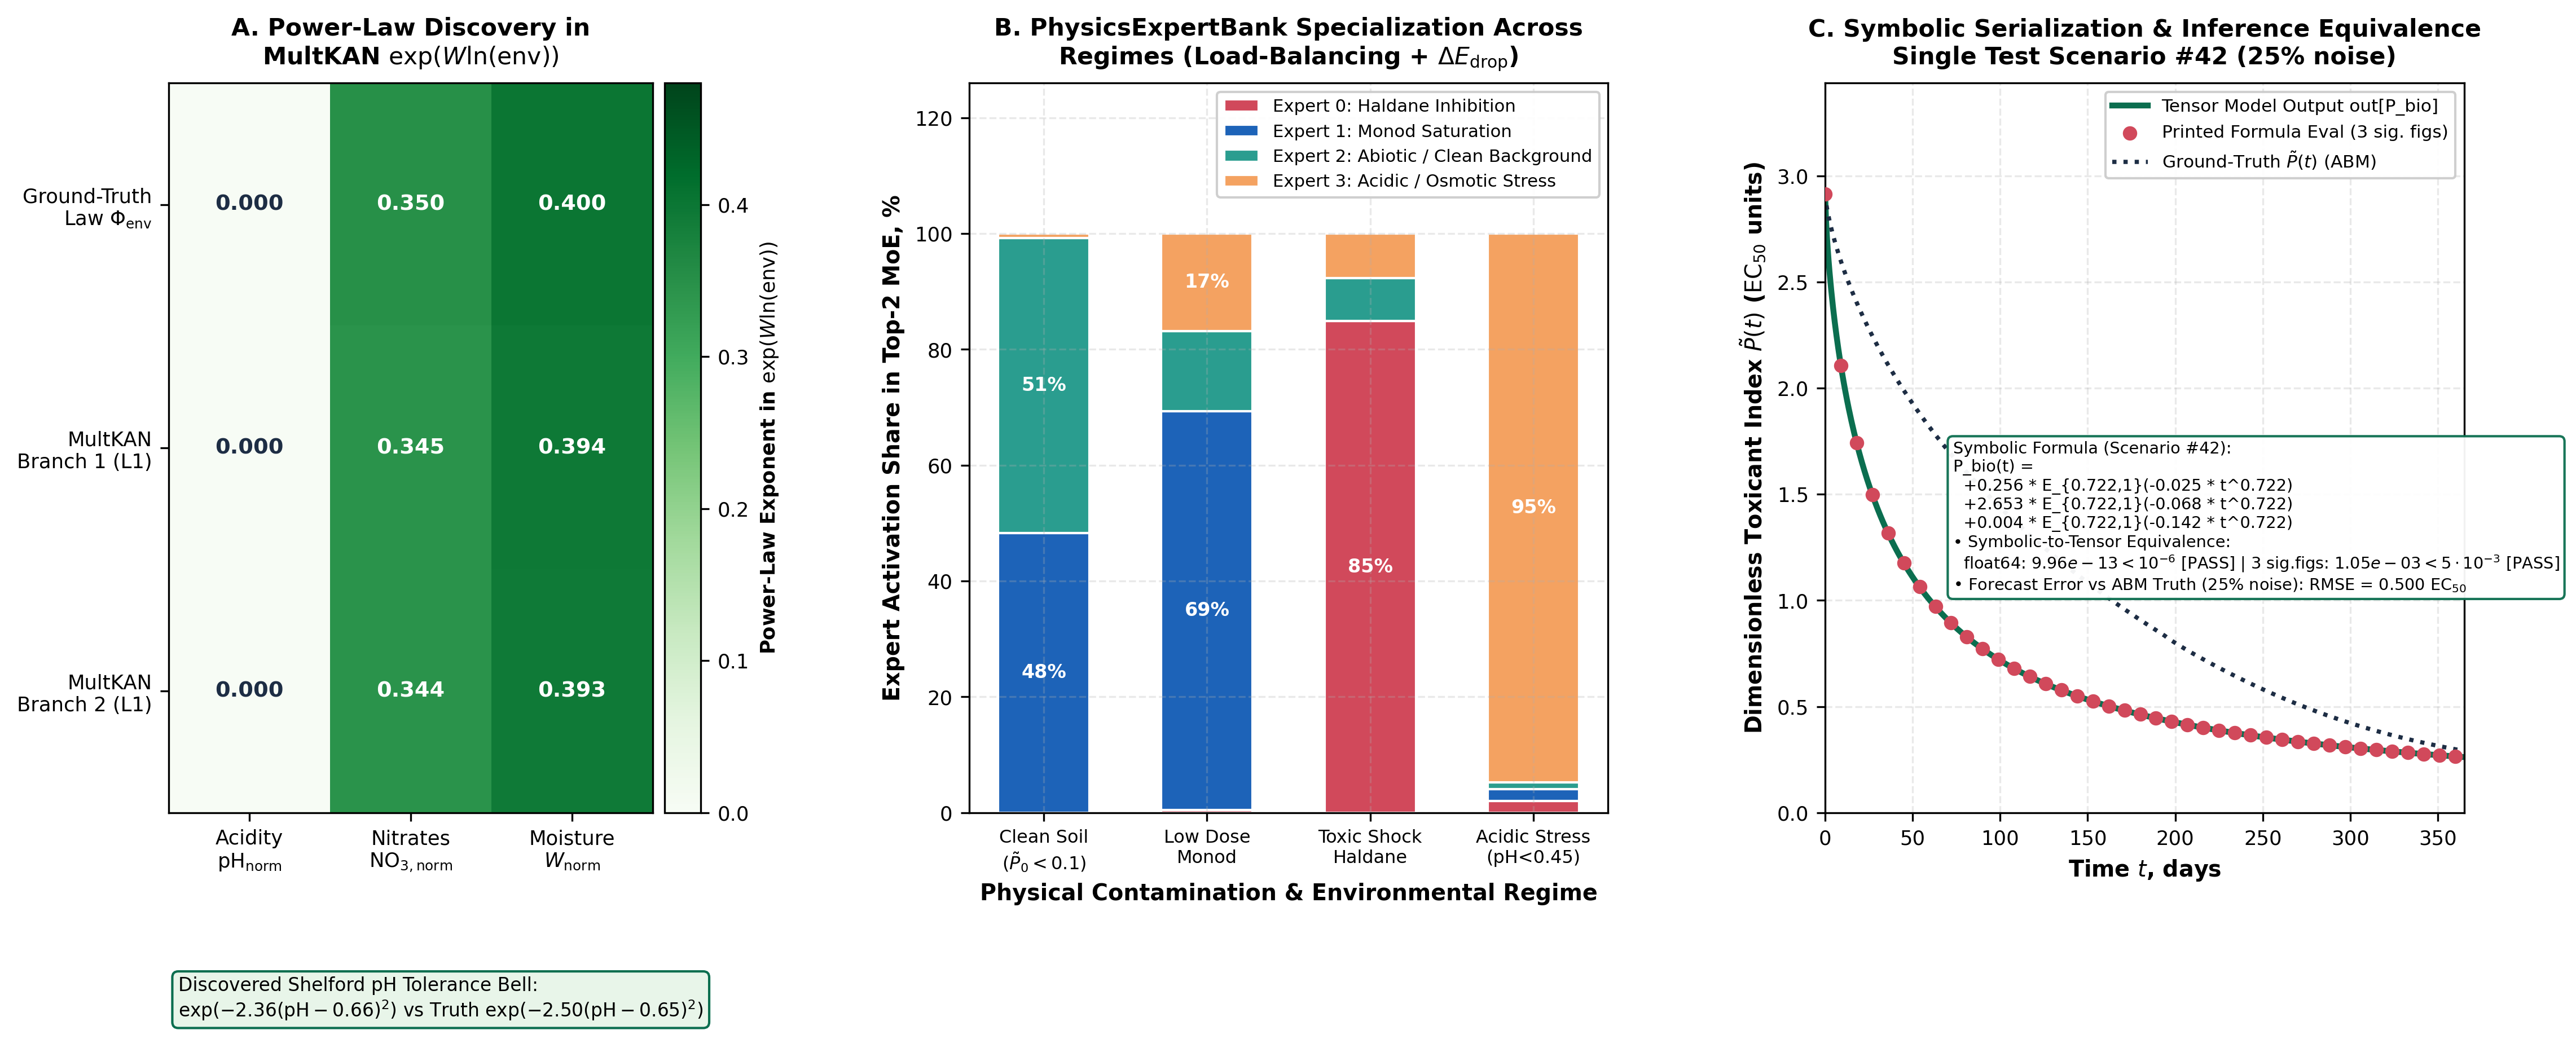
\includegraphics[width=0.95\textwidth]{fig5_multkan_symbolic_discovery.png}
  \vspace{-1mm}
  \caption{\textbf{Neuro-Symbolic Power-Law Discovery (\texttt{MultKAN}), Biokinetic MoE Routing, and Symbolic Serialization Equivalence Check.} \textbf{(A)} Recovery of nitrate ($0.345$) and moisture ($0.394$) exponents and Shelford pH bell. \textbf{(B)} Top-2 expert utilization across 4 regimes. \textbf{(C)} Equivalence between unpacked Mittag-Leffler strings and neural tensor output ($9.96\times 10^{-13}$ in \texttt{float64}).}
  \label{fig:fig5}
\end{figure*}

\begin{figure*}[!htbp]
  \centering
  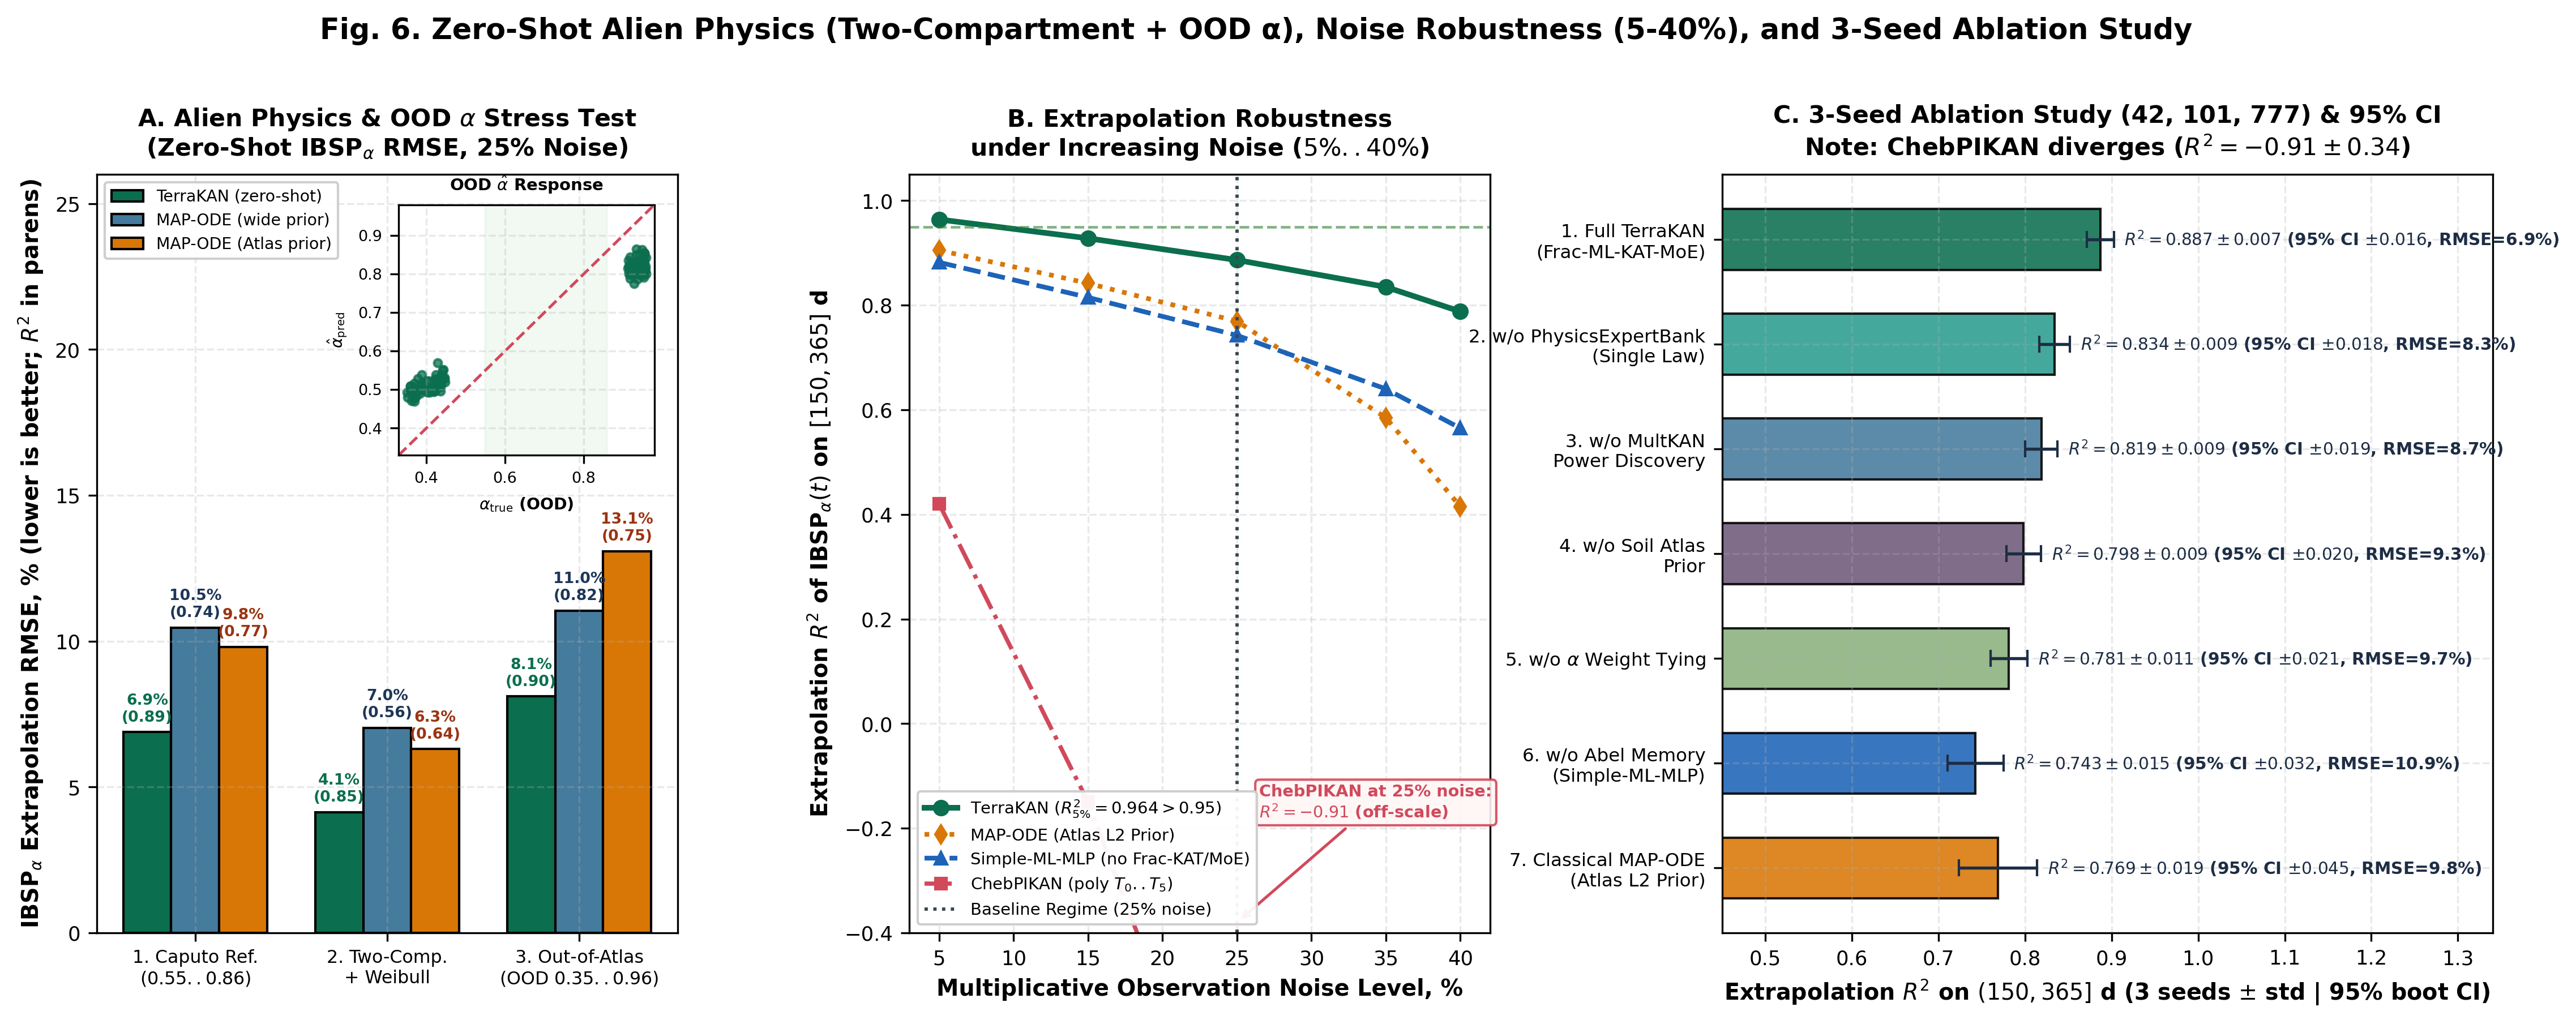
\includegraphics[width=0.95\textwidth]{fig6_ablation_and_noise_robustness.png}
  \vspace{-1mm}
  \caption{\textbf{Zero-Shot Alien Physics (Two-Compartment + OOD $\alpha$, Panel A), Noise Robustness ($5\text{--}40\%$, Panel B), and 3-Seed Ablation Study (Panel C).}}
  \label{fig:fig6}
\end{figure*}

\begin{figure*}[!htbp]
  \centering
  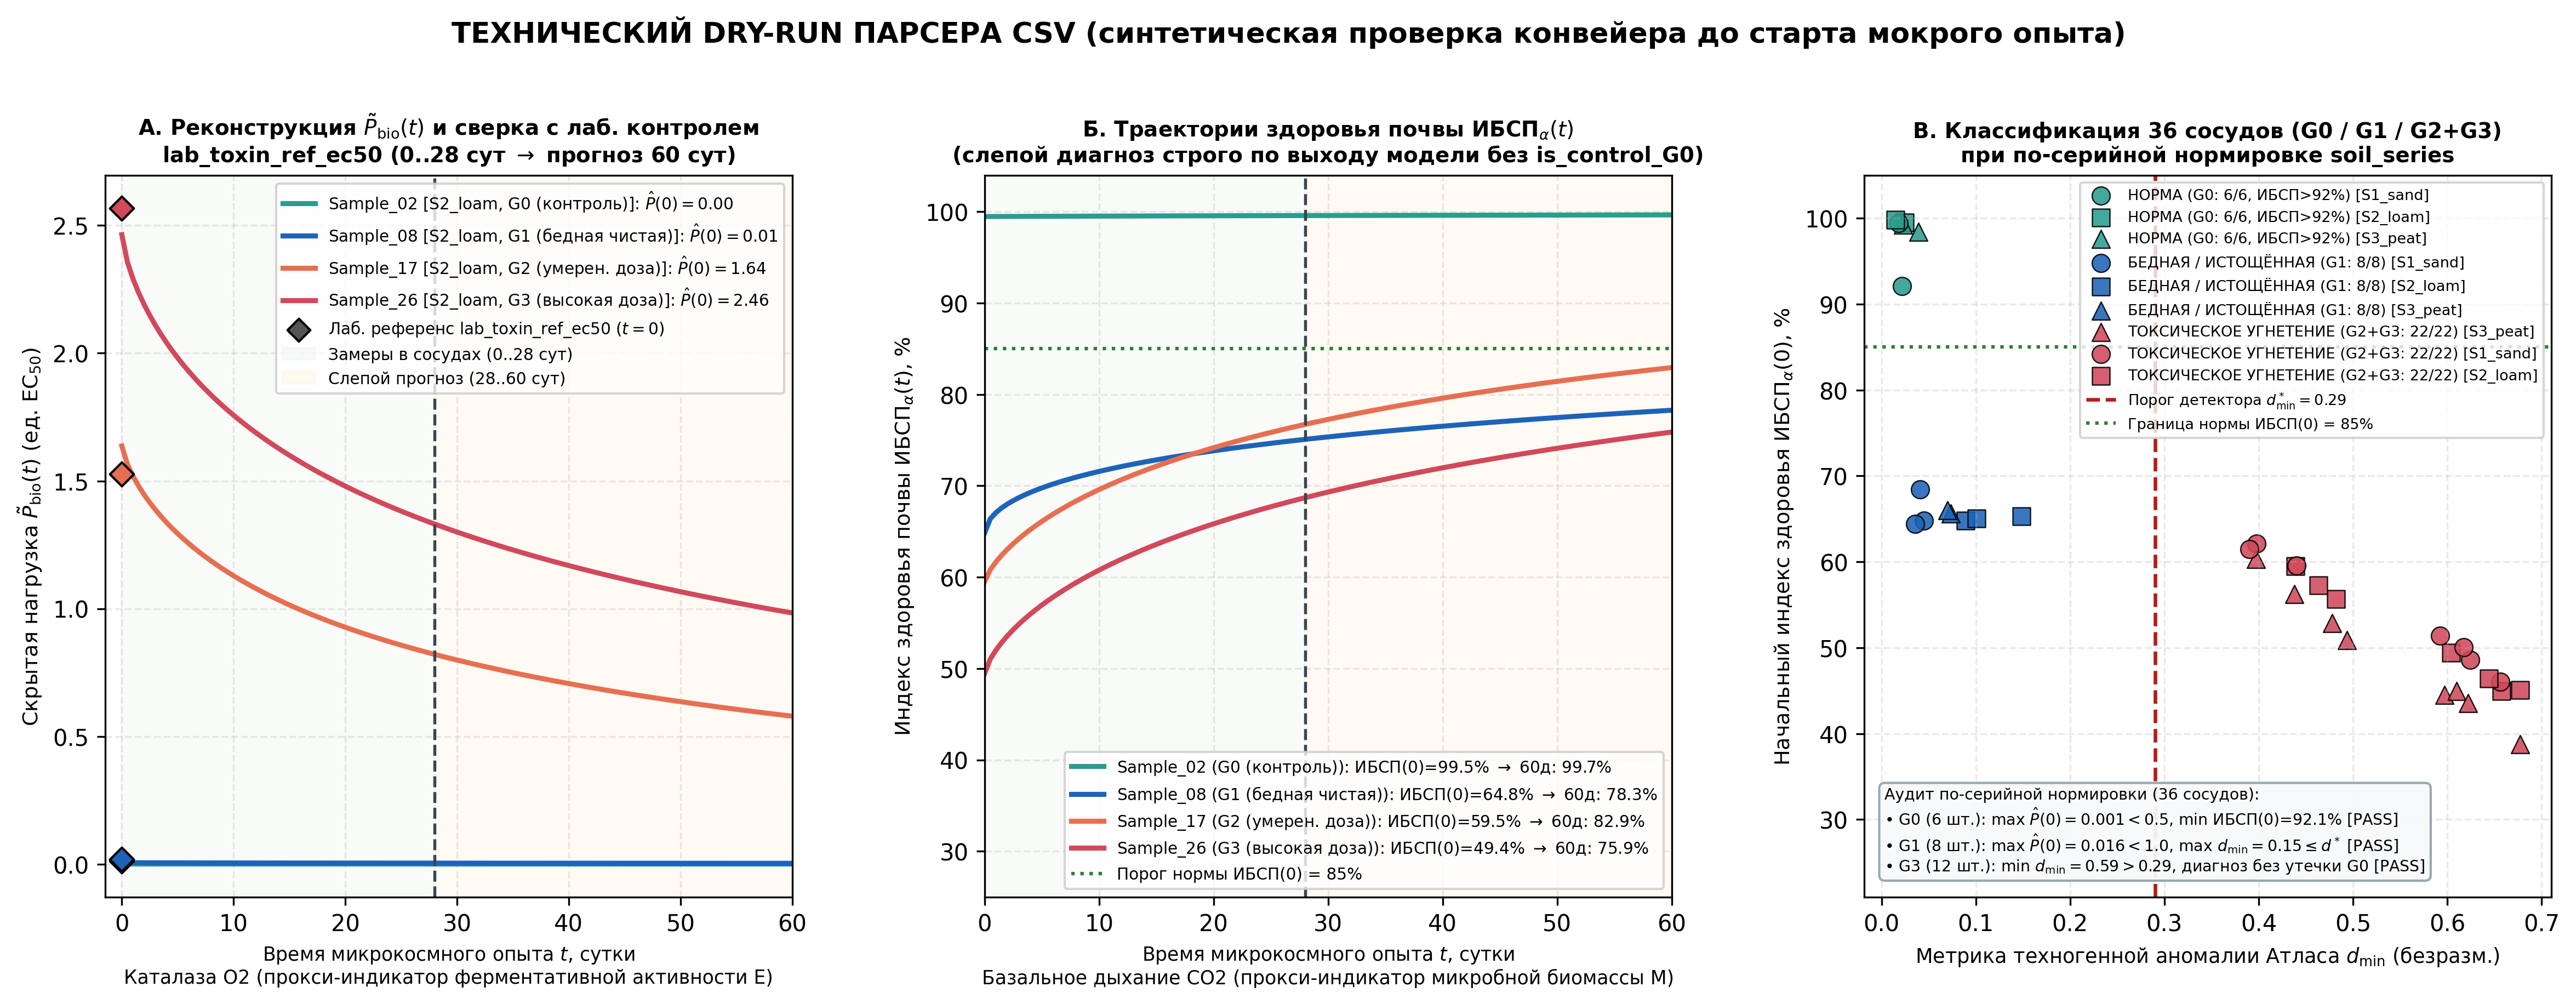
\includegraphics[width=0.95\textwidth]{fig_dry_run_36pots.png}
  \vspace{-1mm}
  \caption{\textbf{Synthetic Dry-Run Verification of Frozen Checkpoint \texttt{terrakan\_v4\_frozen.pt} on 36 Simulated Microcosm Vessels ($0\dots 28\text{ d} \to 60\text{ d}$).} Per-series control normalization (\texttt{S1\_sand}, \texttt{S2\_loam}, \texttt{S3\_peat}) and strictly model-driven diagnosis without \texttt{is\_control\_G0} leakage.}
  \label{fig:fig7}
\end{figure*}

\begin{figure*}[!htbp]
  \centering
  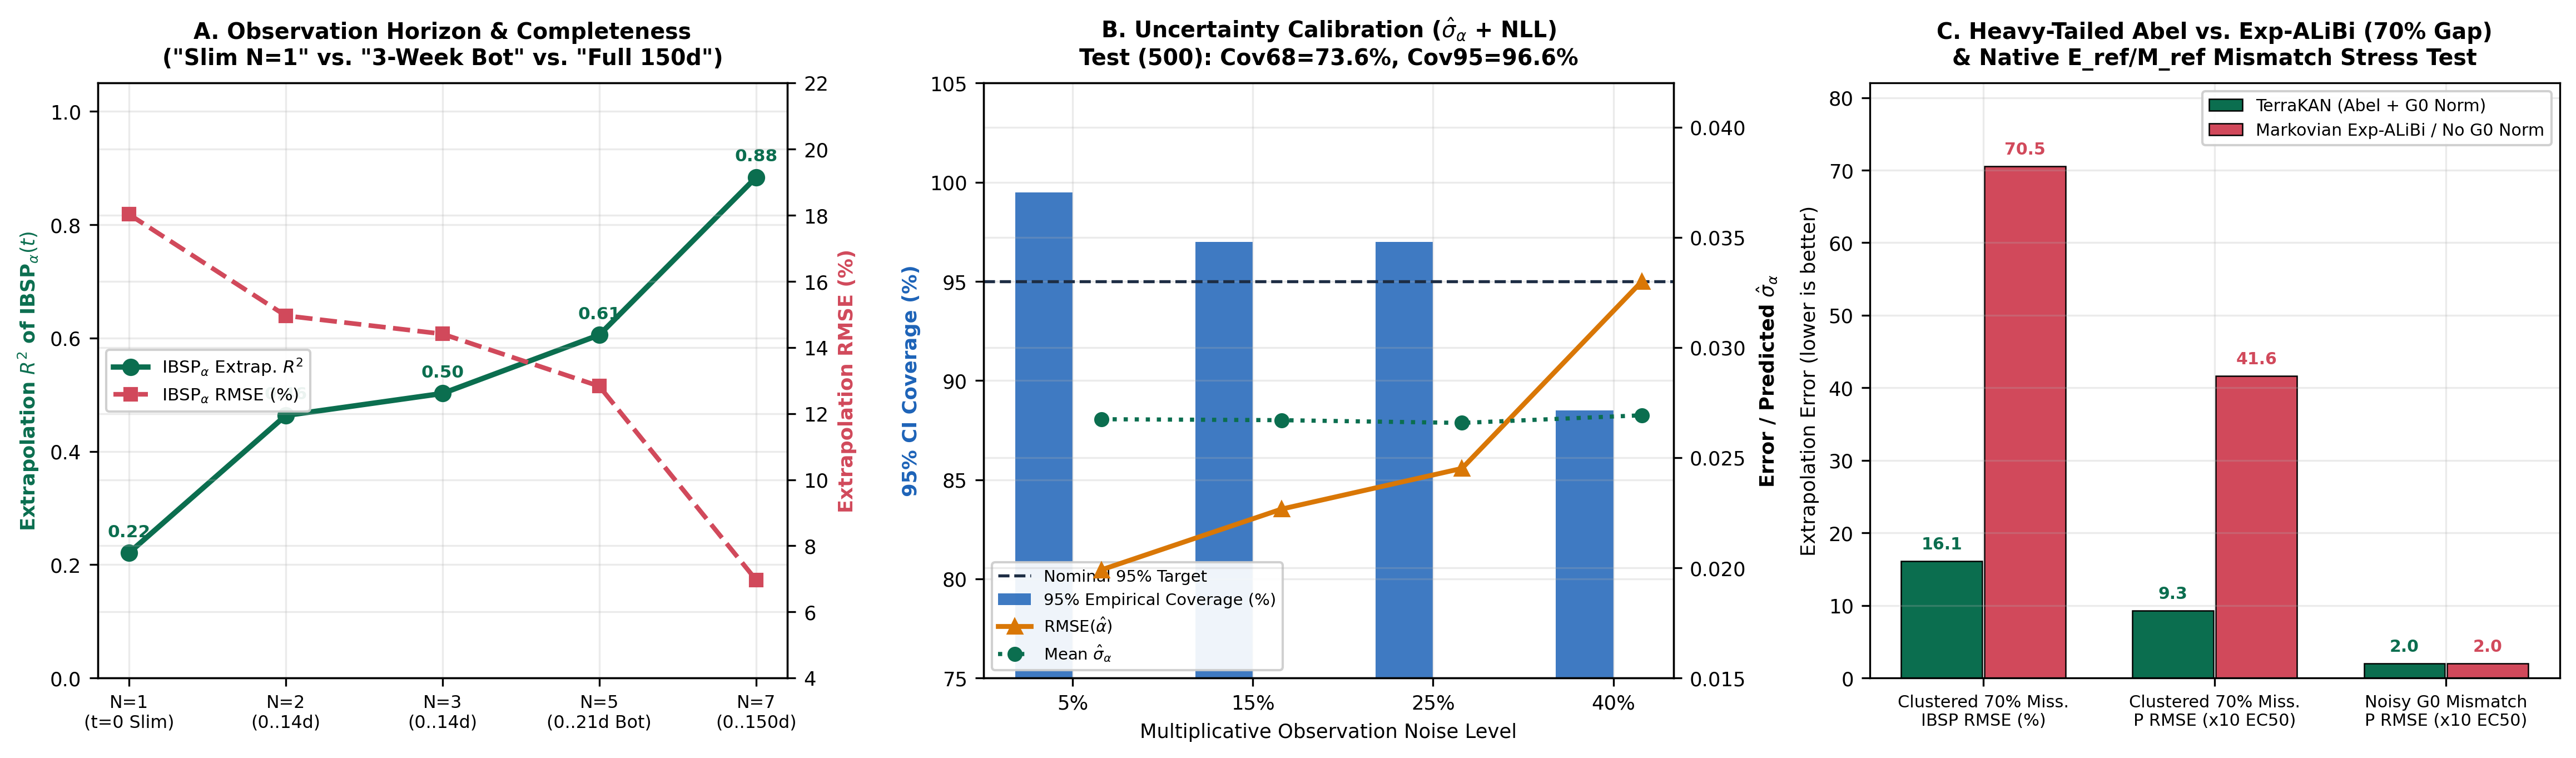
\includegraphics[width=0.95\textwidth]{fig8_v110_horizon_uncertainty.png}
  \vspace{-1mm}
  \caption{\textbf{Operational Horizon Completeness, Uncertainty Calibration, and Heavy-Tailed Memory Audits.} \textbf{(A)} Monotonic accuracy transition from single-visit Slim ($N=1$) to 21-day ($N=5$) and 150-day ($N=7$) regimes. \textbf{(B)} Empirical $95\%$ coverage of $\hat{\sigma}_\alpha$ across $5\%\text{--}40\%$ noise. \textbf{(C)} Abel power-law vs.\ Markovian \texttt{Exp-ALiBi} under $70\%$ clustered missingness and noisy \texttt{G0} scale-mismatch.}
  \label{fig:fig8}
\end{figure*}

\subsection*{AI Usage Disclosure}
During manuscript preparation and code engineering, I used AI-assisted tooling for LaTeX typesetting, refactoring, and automated unit-test scaffolding; all mathematical derivations, model architecture design, simulation experiments, and scientific claims were authored, executed, and verified by me.

\clearpage
\appendix
\section{Simulator Constants \& Baseline Hyperparameters}
In Eqs.~\eqref{eq:caputo_p}--\eqref{eq:caputo_e}, $K_i \equiv 1.0$, $\beta_E = 0.09$, $\delta_E = 0.075$ ($E_{\text{ref}}/M_{\text{ref}} = 1.20$), $\gamma_p \in [0.011, 0.022]$, $\mu_{\text{sub}} \in [0.030, 0.058]$, and $K_s \in [0.80, 1.15]$ (Table~\ref{tab:soil_atlas}). Rainfall pulses ($r_j=1$, probability $0.18$) transiently modulate moisture $W_{\text{norm}}$. All neural baselines (\texttt{TerraKAN}, \texttt{ChebPIKAN}, \texttt{Latent-ODE} [$18,152$ params, 38-step RK4], \texttt{DeepONet} [$40,515$ params, $128$-wide branch / $64$-wide trunk]) are trained for $160$ epochs on CPU (\texttt{float64}, \texttt{Adam}, $\text{lr}=2.5\times 10^{-3}$, batch size $64$).

\section{Proofs of Propositions 1 and 2}
\noindent\textbf{Proof of Proposition 1.} Across $501$ uniformly spaced $\alpha \in [0.40, 0.90]$, the exact linear solve of Eq.~\eqref{eq:pade_system} yields $\min q_1 = 0.9777$, $\min q_2 = 0.4342$, $\min q_3 = 0.1095$, and $\min q_4 = 0.0146 > 0$. Since $Q_4(z) = 1 + \sum_{k=1}^4 q_k z^k$ has zero sign changes, Descartes' Rule of Signs guarantees zero positive real roots on $[0, +\infty)$. Moreover, $Q_4'(z) > 0$ for all $z \ge 0$, so $\min_{z\ge 0} Q_4(z) = Q_4(0) = 1.000000$. At $\alpha=0.90$, $w(0)=w'(0)=0$ and at $\alpha=1.0$, $w(1)=1, w'(1)=0$ for $w(s)=3s^2-2s^3$, ensuring $C^1$ continuity. $\square$

\noindent\textbf{Proof of Proposition 2.} Substituting $\tilde{P} = P / K_{\text{tox}}$ and rescaling $(K_i, K_s) \mapsto (cK_i, cK_s)$ with $(\gamma_p, \mu_{\text{sub}}) \mapsto (\gamma_p/c, \mu_{\text{sub}}/c)$ leaves $M(t)$ and $E(t)$ unchanged in Eqs.~\eqref{eq:caputo_p}--\eqref{eq:caputo_e}. Fixing $K_{\text{tox}} \equiv K_i \equiv 1.0$ eliminates $c$, and Eq.~\eqref{eq:p0_boundary} uniquely determines $\tilde{P}(0)$ whenever $E_{\text{ref}}/M_{\text{ref}}$ is known or calibrated via \texttt{G0}. $\square$


\begin{figure*}[!htbp]
\centering
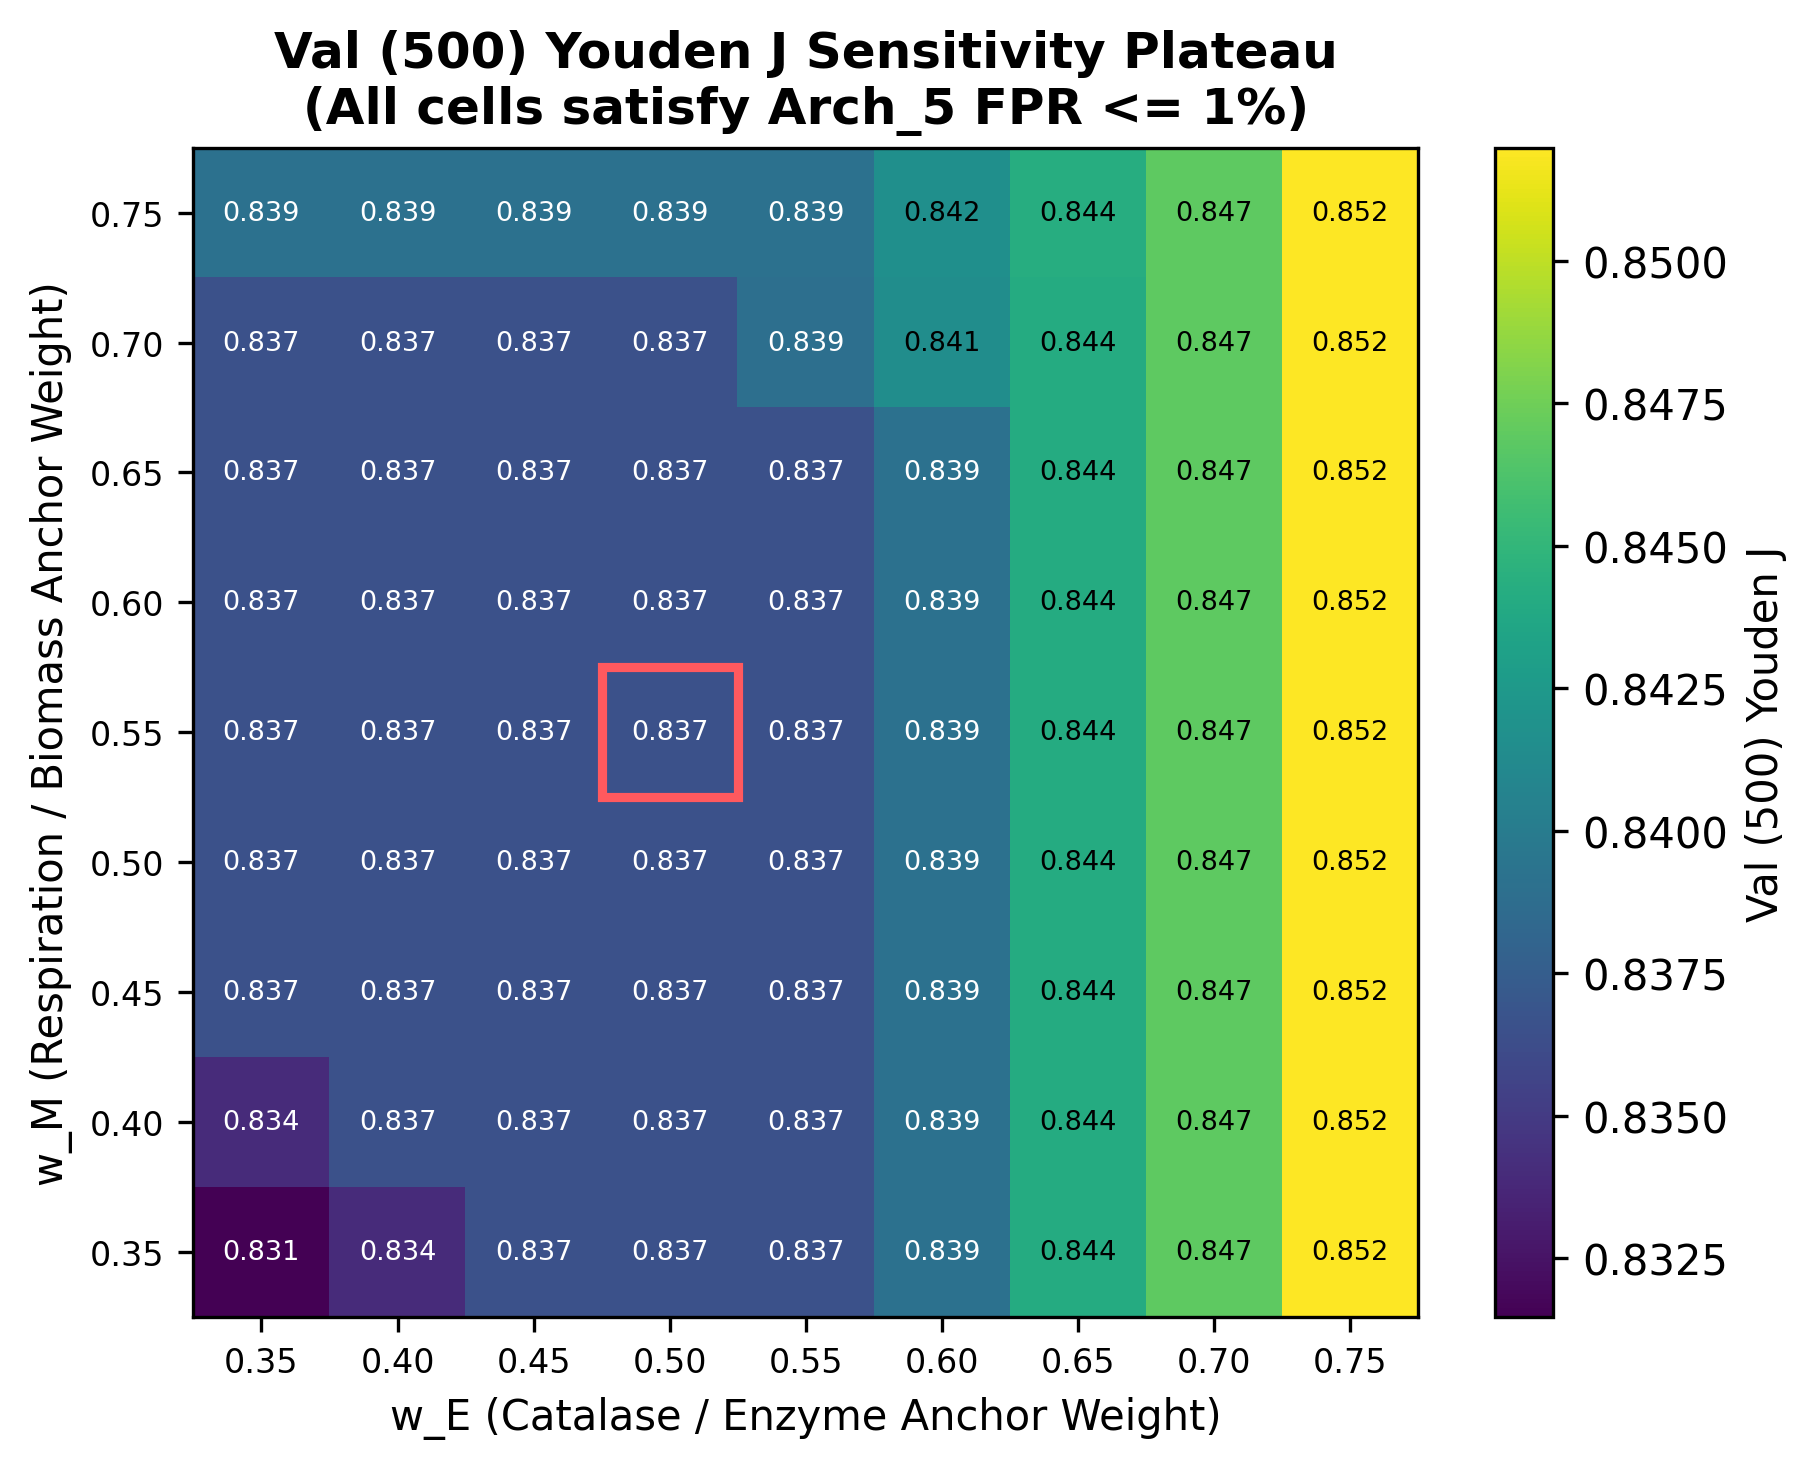
\includegraphics[width=0.62\textwidth]{fig_v125_wm_we_heatmap.png}
\caption{\textbf{Val (500) Sensitivity Heatmap for $(w_M, w_E) \in [0.35, 0.75]^2$.} Youden's $J$ forms a broad plateau ($[0.8315, 0.8520]$) around $(0.55, 0.50)$ (red box).}
\label{fig:v125_hm}
\end{figure*}

\clearpage
\begin{thebibliography}{14}
\footnotesize
\setlength{\itemsep}{1.5pt}

\bibitem{tu2026fractional}
Tu, W., Liu, X., Wang, H., Li, X., \& Han, C. (2026). Fractional Calculus for Large Language Models: A Survey of Potentials, Mechanisms, and Challenges. \textit{Fractal and Fractional}, 10(7), 454. \href{https://doi.org/10.3390/fractalfract10070454}{https://doi.org/10.3390/fractalfract10070454}

\bibitem{liu2024kan}
Liu, Z., Wang, Y., Vaidya, S., et al. (2024). KAN: Kolmogorov-Arnold Networks. \textit{arXiv preprint} \href{https://arxiv.org/abs/2404.19756}{arXiv:2404.19756}.

\bibitem{liu2024kan2}
Liu, Z., Ma, P., Wang, Y., Matusik, W., \& Tegmark, M. (2024). KAN 2.0: Kolmogorov-Arnold Networks Meet Science (\texttt{MultKAN}). \textit{arXiv preprint} \href{https://arxiv.org/abs/2408.10205}{arXiv:2408.10205}.

\bibitem{yang2025kat}
Yang, X., \& Wang, X. (2025). Kolmogorov-Arnold Transformer. \textit{International Conference on Learning Representations (ICLR 2025)} / \href{https://arxiv.org/abs/2409.10594}{arXiv:2409.10594}.

\bibitem{aghaei2024rkan}
Aghaei, A. A. (2024). rKAN: Rational Kolmogorov-Arnold Networks. \textit{arXiv preprint} \href{https://arxiv.org/abs/2406.14495}{arXiv:2406.14495}.

\bibitem{zeng2015}
Zeng, C., \& Chen, Y. (2015). Global Pad\'e approximations of the generalized Mittag-Leffler function and its inverse. \textit{Fractional Calculus and Applied Analysis}, 18(6), 1492--1506. \href{https://arxiv.org/abs/1310.5592}{arXiv:1310.5592}

\bibitem{schumer2003}
Schumer, R., Benson, D. A., Meerschaert, M. M., \& Baeumer, B. (2003). Fractal mobile/immobile solute transport. \textit{Water Resources Research}, 39(10), 1296. \href{https://doi.org/10.1029/2003WR002141}{https://doi.org/10.1029/2003WR002141}

\bibitem{aghaei2024fkan}
Aghaei, A. A. (2024). fKAN: Fractional Kolmogorov-Arnold Networks with trainable Jacobi basis functions. \textit{arXiv preprint} \href{https://arxiv.org/abs/2406.07456}{arXiv:2406.07456}.

\bibitem{abueidda2025deepokan}
Abueidda, D. W., Pantidis, P., \& Mobasher, M. E. (2025). DeepOKAN: Deep Operator Network Based on Kolmogorov Arnold Networks for Mechanics Problems. \textit{Computer Methods in Applied Mechanics and Engineering}, 436, 117699. \href{https://doi.org/10.1016/j.cma.2024.117699}{https://doi.org/10.1016/j.cma.2024.117699}

\bibitem{kolesnikov2021ag}
Kolesnikov, S., Timoshenko, A., Minnikova, T., Tsepina, N., Kazeev, K., Akimenko, Y., Zhadobin, A., Shuvaeva, V., Rajput, V. D., Mandzhieva, S., \& Minkina, T. (2021). Influence of Silver Nanoparticles on the Biological Indicators of Haplic Chernozem. \textit{Plants}, 10(5), 1022. \href{https://doi.org/10.3390/plants10051022}{https://doi.org/10.3390/plants10051022}

\bibitem{mdpienzymes2024}
Minnikova, T., Kolesnikov, S., Kuzina, A., Trufanov, D., Khrapay, E., \& Trushkov, A. (2024). Enzymatic Diagnostics of Soil Health of the European Part of Russia with Lead Contamination. \textit{Soil Systems}, 8(3), 76. \href{https://doi.org/10.3390/soilsystems8030076}{https://doi.org/10.3390/soilsystems8030076}

\bibitem{mdpi2024oxidoreductases}
Wyszkowska, J., et al. (2024). The Potential for Restoring the Activity of Oxidoreductases and Hydrolases in Soils Contaminated with Petroleum Products. \textit{Applied Sciences}, 14(9), 3591. \href{https://doi.org/10.3390/app14093591}{https://doi.org/10.3390/app14093591}

\bibitem{diethelm2002predictor}
Diethelm, K., Ford, N. J., \& Freed, A. D. (2002). A predictor-corrector approach for the numerical solution of fractional differential equations. \textit{Nonlinear Dynamics}, 29, 3--22. \href{https://doi.org/10.1023/A:1016592219341}{https://doi.org/10.1023/A:1016592219341}

\bibitem{kazeev2003bio}
Kazeev, K. Sh., Kolesnikov, S. I., \& Valkov, V. F. (2003). \textit{Biological Diagnostics and Indication of Soils: Methodology and Research Methods} [in Russian]. Rostov-on-Don: Southern Federal University Press.

\bibitem{margesin2001} R. Margesin and F. Schinner, ``Bioremediation (natural attenuation and biostimulation) of diesel-oil-contaminated soil in an alpine glacier skiing area,'' \textit{Appl. Environ. Microbiol.}, vol. 67, no. 7, pp. 3127--3133, 2001. \url{https://pmc.ncbi.nlm.nih.gov/articles/PMC92991/}
\bibitem{garousin2021} H. Garousin et al., ``Effects of bioaugmentation and biostimulation on $>60$-year-old petroleum-contaminated saline-sodic soil,'' \textit{Front. Microbiol.}, vol. 12, 642215, 2021. \href{https://doi.org/10.3389/fmicb.2021.642215}{https://doi.org/10.3389/fmicb.2021.642215}
\bibitem{chai2023} X. Chai et al., ``Shift of combined ecotoxicity index in petroleum polluted soils during a bacterial remediation,'' \textit{Front. Environ. Sci.}, vol. 11, 1141562, 2023. \href{https://doi.org/10.3389/fenvs.2023.1141562}{https://doi.org/10.3389/fenvs.2023.1141562}
\bibitem{rafikova2026} G. Rafikova et al., ``Effects of salinization, oil contamination, and heavy metals on soil biological activity and phytoremediants,'' \textit{Toxics}, vol. 14, no. 2, 186, 2026. \href{https://doi.org/10.3390/toxics14020186}{https://doi.org/10.3390/toxics14020186}
\end{thebibliography}

\end{document}
